% !TeX root = ../thuthesis-example.tex

\chapter{指环上的高准确低延迟触摸检测技术}\label{section:TappingRing}

\section{引言}

头戴式混合现实设备(MR头盔,如微软的Hololens\cite{hololens2})为新一代人机交互范式带来了丰富的可能性。MR头盔通过前置深度摄像头感知物理环境和用户动作,通过带有显示器护目镜将三维虚拟元素渲染在物理实体之上,原则上使得MR头盔用户可以随时随地与数字世界交互。MR头盔上一种也有前景、有价值的应用场景是在无源表面(如桌面、墙面)上投射虚拟用户界面,并允许人通过触摸与用户界面进行交互。上述应用场景将触摸交互——当前用户规模最大的人机交互方式,从有源触摸屏的束缚中解放出来,拓展到任意物理表面上。与目前MR头盔上流行的空中手势交互相比,触摸交互提供真实的触觉反馈,这是自然人机交互体验的重要组成部分。

要在MR头盔情境下检测无源表面的触摸交互,一个直观的想法是利用MR头盔的前置深度摄像头,通过视觉方法检测触摸事件。然而,视觉方法在检测触摸交互时存在固有的缺陷:首先,由于摄像头在手背的方向,摄像头在捕捉手指接触交互表面时面临严重的遮挡问题,在大多数情况下,摄像头都无法直接观察到手指接触交互表面的位置;第二,目前主流的深度摄像头是基于双目视觉的,这一类型的深度摄像头在识别交互表面的深度时精度不高,特别是当交互表面是纯色的、无明显视觉关键点的时候,误差可能达到厘米级别,对触摸交互技术的响应性带来很大挑战;第三,视觉方法的计算过程复杂,在计算资源有限的机器上运算可能会带来用户难以接受的延迟。例如,在利用视觉方法检测无源表面触摸交互的代表性工作MRTouch\cite{xiao2018mrtouch}中,研究者利用Hololens混合现实头盔的前置摄像头检测触摸事件,其未识别率高达3.5\%,误触率高达19.0\%,端到端延迟高达180 毫秒。这说明,基于视觉方法的无源表面触摸交互技术仍需改进。

\begin{figure}
	\centering
	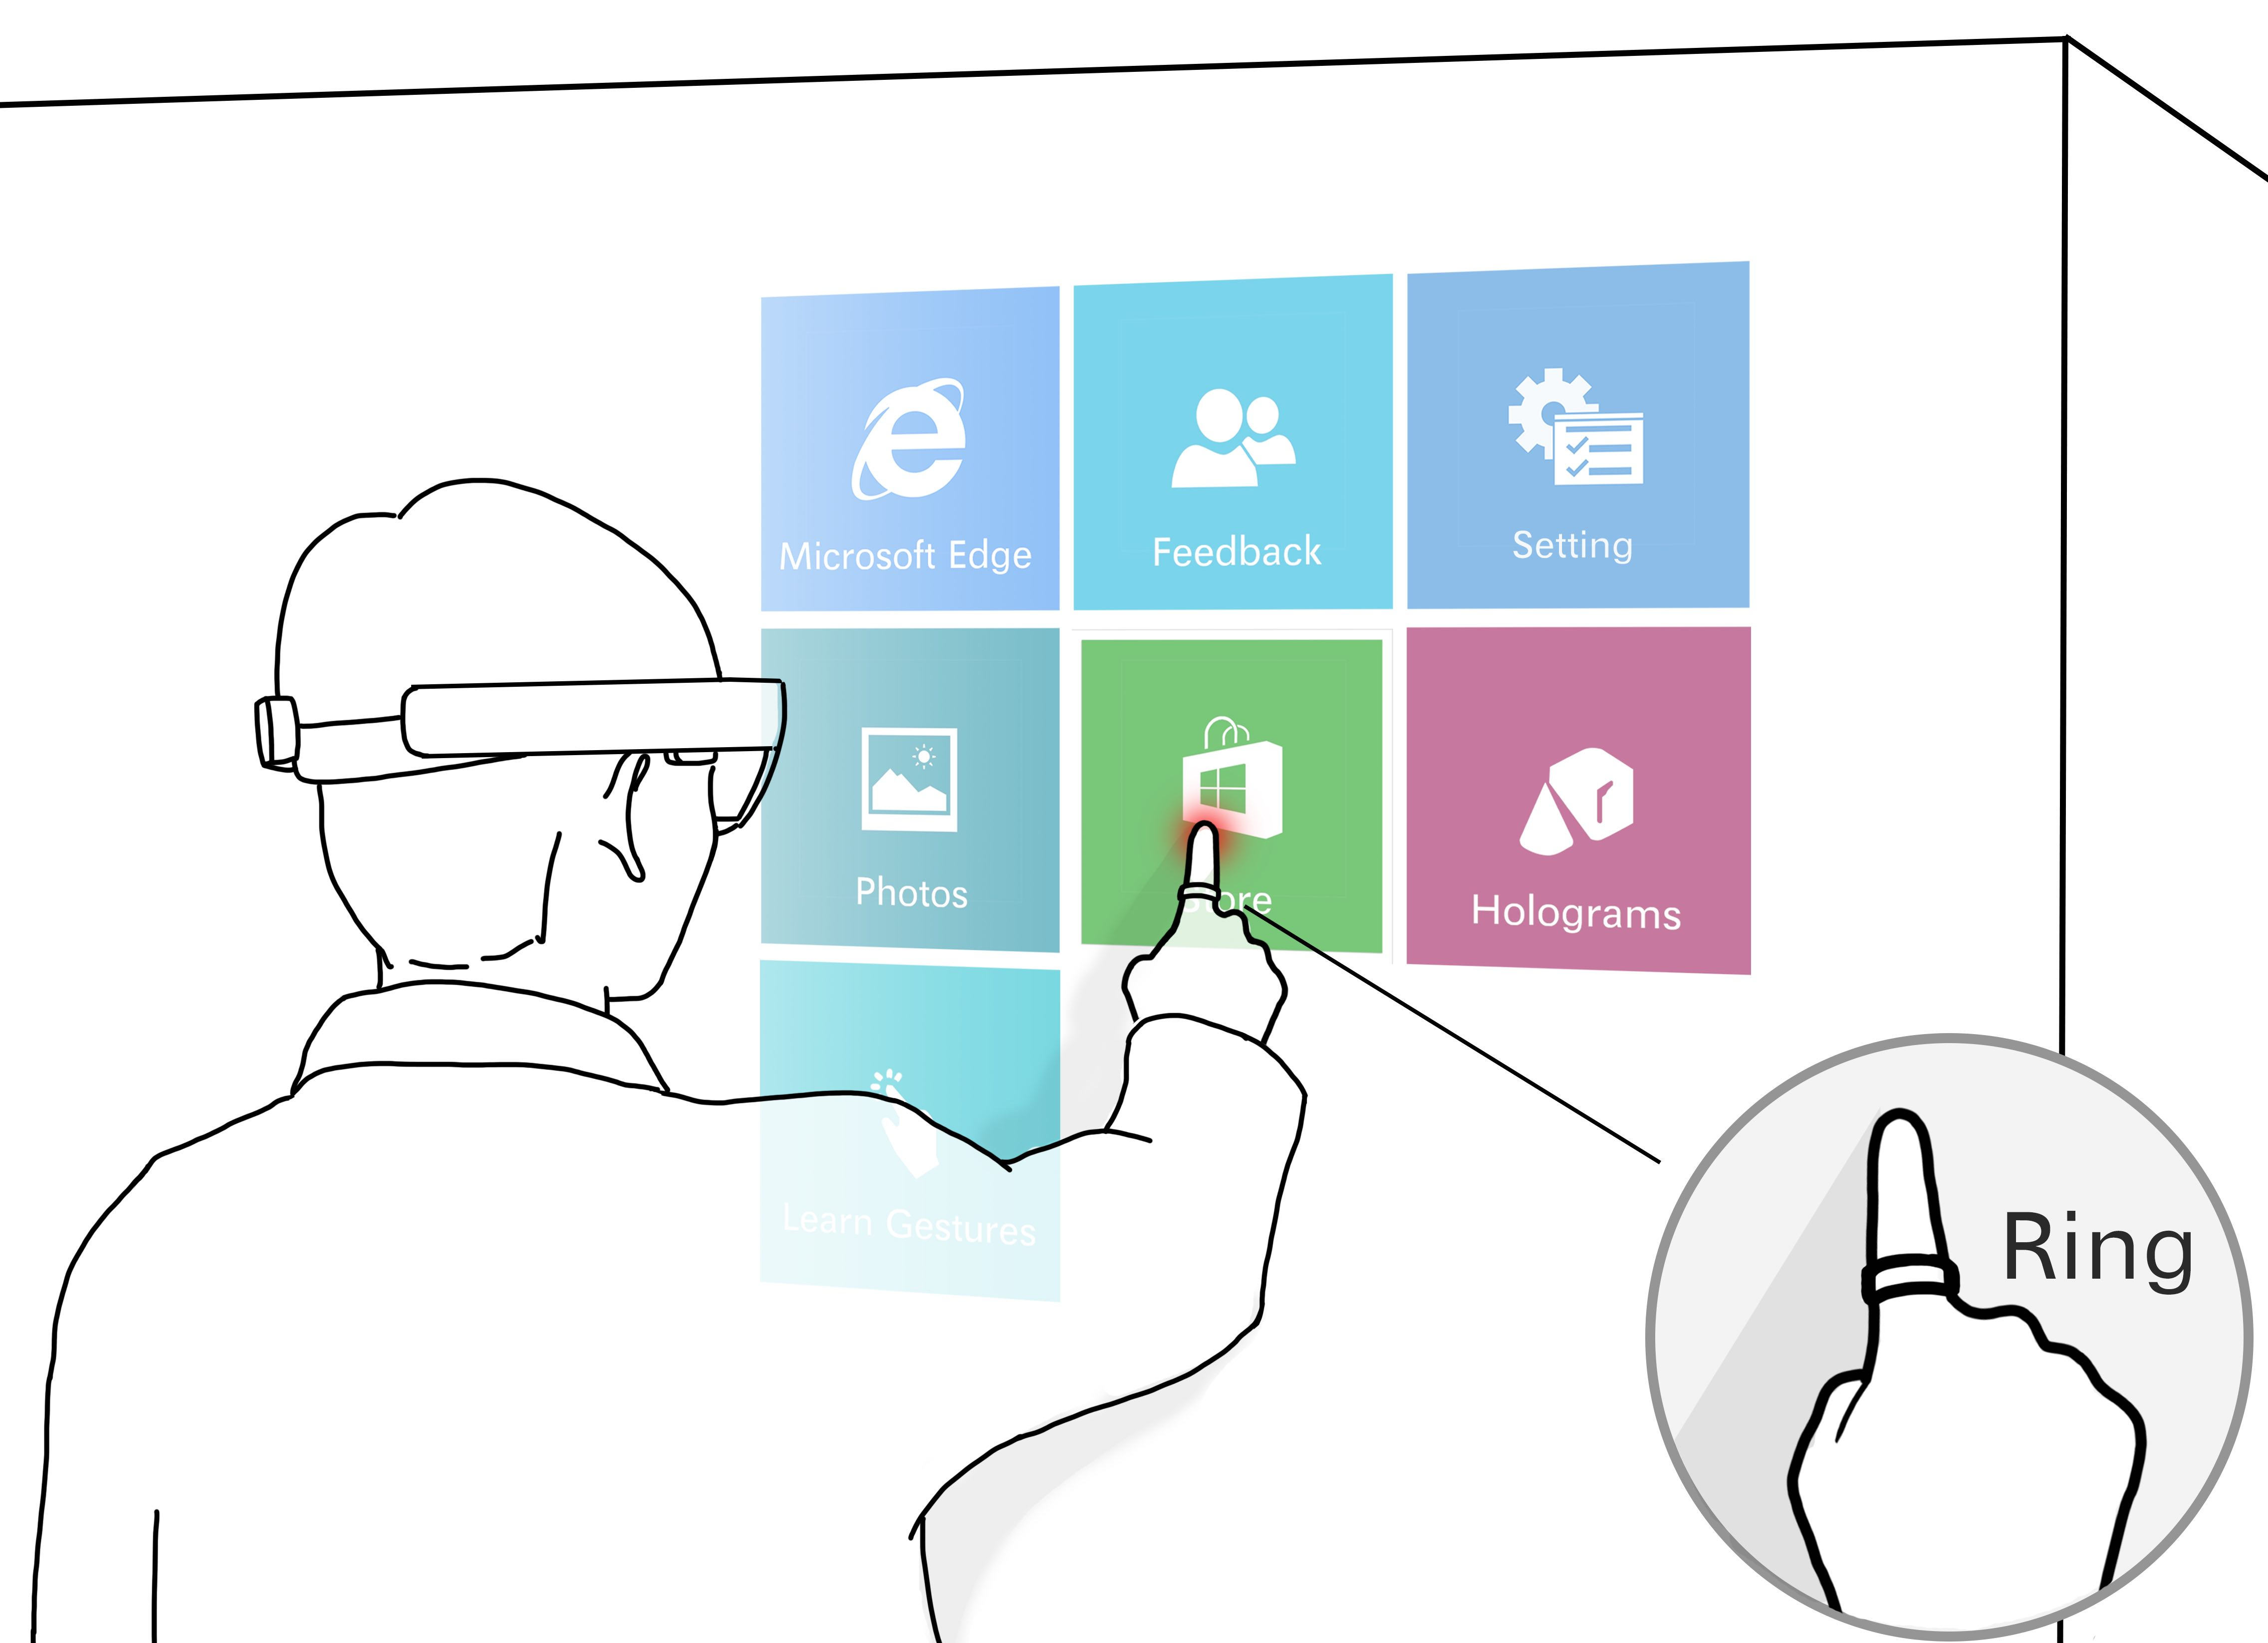
\includegraphics[width=0.8\linewidth]{MR_touch_envision.jpg}
	\caption*{结合MR头盔和智能指环有望在无源表面上支持流畅的触摸交互体验。}
	\caption{MR场景下触摸交互无处不在的设想}
	\label{fig:MR_touch_envision2}
\end{figure}

如图\ref{fig:MR_touch_envision2}所示,我们设想在未来结合MR头盔和智能指环来使能无源表面上流畅的触摸交互体验:MR头盔的前置摄像头主要负责识别手指的2D位置和姿态,而戴在手指上的惯性传感指环主要负责低延迟地检测手指是否接触到了交互表面。由于惯性传感器所提供的数据带宽较低,处理惯性传感器数据的计算通常是高效的,这确保了触摸检测的高响应性。在相关文献中,先前的工作已经探索过使用手指上佩戴的惯性传感器来增强触摸交互技术\cite{lam2002mids, oh2017anywheretouch, masson2017whichfingers}。使用智能指环感知触摸并不是本文的创新点,然而,先前工作仅对惯性传感器信号使用阈值方法来检测触摸事件,其响应性非常低下(准确率不超过89.8\%,延迟不低于50毫秒),因此基于惯性传感指环的触摸交互技术还有很大的改进空间。

为提高指环触摸交互技术的可用性,本文提出了基于惯性传感指环的低延迟触摸检测技术。低延迟是该技术与先前工作的主要区别,该技术的检测延迟低至10毫秒,而人无法在触摸交互中察觉到10毫秒的延迟,因此该技术在响应性上提供了最佳的用户体验。本章将从各个维度介绍基于惯性传感指环的低延迟触摸检测技术:

首先,本章开展了两项用户实验来调研触摸交互指环的设计问题,分别是用户对不同触摸姿态的主观喜好程度调研(实验一A),和用户对不同指环佩戴位置的主观喜好程度调研(实验一B),这两项实验的结果将指导技术的交互设计。然后,本章通过用户实验采集用户佩戴智能指环进行触摸交互的数据(实验二),再利用简单的机器学习方法实现了初版的触摸检测技术,用于对比指环佩戴在不同位置上时触摸交互技术的性能。最后,本章将触摸运动模型应用在指环触摸交互技术的改进上,介绍了基于基于惯性传感指环的低延迟触摸检测技术。评测实验(实验三)的结果显示,该技术的触摸检测准确率高达98.61\%(精确度98.61\%,召回率98.62\%),检测延迟低至10毫秒。这一结果说明,基于惯性传感指环的低延迟触摸检测技术具有高响应性,同时,该技术因支持无源表面触摸交互而具有高普适性,是一项有着广阔应用前景的新技术。

\section{相关工作}

本文引言已经提到,触摸交互技术主要分为有源触摸屏技术和无源表面触摸技术两大类。有源触摸屏技术是目前最常用的触摸交互技术\cite{lee1985multi, wang2009empirical, wilson2004touchlight},但由于它被束缚在有源表面上的内禀缺陷,触摸屏技术始终不具备适应未来穿戴计算交互模态的普适性。在MR头盔等新型交互设备兴起的背景之下,无源表面触摸交互技术是有前景的研究方向。无源表面触摸交互主要有种技术实现方案,基于摄像头的视觉方法和基于震动的方法,这两种方法在本质上分别对应触摸运动的位移信号和加速度信号。

\subsection{基于视觉的无源表面触摸交互}

摄像头可以通过视觉方法观察手指触碰交互表面的时间和位置,从而检测触摸事件,支持触摸交互。当摄像头部署在场景空间中,或作为可穿戴设备部署在人身上\cite{harrison2011omnitouch, xiao2018mrtouch},而非直接部署在交互表面上时,即可认为摄像头支持无源表面上的触摸交互,具有较高的普适性。在相关工作中,已有研究者利用激光雷达\cite{paradiso2000sensor}、RGB摄像头\cite{agarwal2007high, chang2005real, letessier2004visual, sugita2008touch}、红外摄像头\cite{grudin2001integrating}、热成像摄像头\cite{saba2012dante}和深度摄像头\cite{agarwal2007high, xiao2016direct, xiao2018mrtouch, benko2012miragetable, harrison2011omnitouch, wilson2010combining}实现基于视觉方法的无源表面触摸交互技术。然而,先前基于视觉的触摸交互技术的基本原理都是直接观察手指是否接触交互表面,这种方法面临严重的遮挡问题,影响了触摸交互技术的响应性,即使在最新工作中\cite{xiao2018mrtouch},该方案的误触率也高达19.0\%,端到端延迟高达180毫秒。本文的触摸运动模型为基于视觉的无源表面触摸交互技术带来了新思路,不同于先前技术中摄像头“直接”观察手指是否触摸表面的思路,触摸运动模型揭示:可以通过手指触摸表面时的瞬停现象“间接”地判断触摸事件,从而有效规避遮挡问题,提高触摸检测的响应性。

\subsection{基于震动的无源表面触摸交互}

在触摸交互中,当手指接触到交互表面上时,会引发手指的震动,并且发出声音。震动和声音可以被惯性传感器和麦克风所捕捉,因此,不少工作致力于探索基于震动的无源表面触摸交互,利用部署在人的手指\cite{gu2019accurate, shi2020ready, gu2020qwertyring}或手腕\cite{meier2021tapld}上的传感器感知触摸。然而,先前工作仅通过阈值方法感知触摸\cite{lam2002mids, oh2017anywheretouch, niikura2014anywhere},即当手指震动幅度或声音响度超过特定阈值时判定触摸发生,其准确率不超过89.8\%,端到端延迟不低于50毫秒,不满足触摸交互的高响应性需求。本文的触摸运动模型为基于震动的无源表面触摸交互技术提供计算理论基础,模型指出,除去手指接触交互表面瞬间引发的震动以外,手指向下过程中的众多运动信号规律都有助于提高触摸检测技术的响应性。在触摸运动模型的基础之上,本文作者在2019年提出基于惯性传感指环的低延迟触摸检测技术\cite{gu2019accurate},亦即本章所介绍的内容,该技术将无源表面触摸交互技术的响应性提升到用户无法察觉到延迟的标准,后来有研究者跟随并改进了这份工作。例如,本文作者和Shi等人在同一时期提出惯性传感指环不仅可用户检测单次触摸事件,还可以识别长按、滑动拖拽等触摸手势\cite{gu2020qwertyring, shi2020ready};Meier等人提出通过两个惯性传感器,可以将设备从手指上转移到手腕上\cite{meier2021tapld},而不会严重影响触摸交互技术的检测性能。

\subsection{触摸姿态}

触摸姿态指的是触摸交互中,人的手指接触交互表面时的全手型姿态,例如,食指指腹点击、中指指尖敲击、食指第二关节叩击、三指触摸都是不同的触摸姿态。触摸交互技术若能区分不同的触摸姿态,将能丰富触摸交互的表达力\cite{cao2008shapetouch, harrison2011tapsense},然而因为目前主流的触摸屏技术无法区分不同的触摸姿态,所以相关研究一直停留在实验室阶段。随着触摸交互技术的发展,触摸姿态的多样化将被相关技术所支撑,这也是本章将就用户对不同触摸姿态的主观喜好程度进行实验调研的动机。除了触摸姿态以外,触摸压力\cite{ramos2004pressure}、速度\cite{heo2011forcetap, iwasaki2009expressive}、切向力\cite{heo2011force}和手指朝向\cite{roudaut2009microrolls, xiao2015estimating}等额外的输入信道也能丰富触摸交互的表达力,可作为未来的研究方向。

\section{指环触摸交互的自然性研究}

由于指环上无源表面触摸交互技术对普通用户而言是陌生的,本章重视该交互方式的自然性研究。为此,本章开展了两项用户实验来探索指环触摸交互的自然性问题,分别调研了用户对不同触摸姿态和不同指环佩戴位置的主观喜好程度,从而指导本智能指环触摸检测技术的交互设计。

\subsection{实验一A:触摸姿态主观喜好程度调研}

本着人机交互以人为中心的原则,好的触摸交互技术应支持用户喜好的触摸姿态,而非易于识别的触摸姿态。为此,实验一A通过实验和问卷调研被试对不同触摸姿态的喜好程度,以寻找触摸交互技术应支持的触摸姿态集合。首先,我们定义了一套触摸姿态全集;然后,对于触摸姿态全集中的每个姿态,我们要求被试分别将水平的桌面和垂直的墙面视为交互表面,使用该姿态进行“触摸”,亲身感受后在问卷中对该触摸姿态进行评分。最后,实验者根据被试的评分选择出最受用户喜好的触摸姿态集合。

\subsubsection{触摸姿态全集}

如图\ref{fig:posture_set}所示,我们通过一个三维的设计空间来探索触摸姿态的全集,这三个维度分别是:

\begin{itemize}
\item \textbf{哪些手指触摸交互表面?}选项包括拇指、食指、中指、无名指、小指、双指和三指。
\item \textbf{手指的哪个部分触摸交互表面?}参考相关工作TapSense\cite{harrison2011tapsense},选项包括指腹、指尖、手指第二关节、指侧和指甲。
\item \textbf{手部状态?}选项包括五指张开和握拳。
\end{itemize}

\begin{figure}
	\centering
	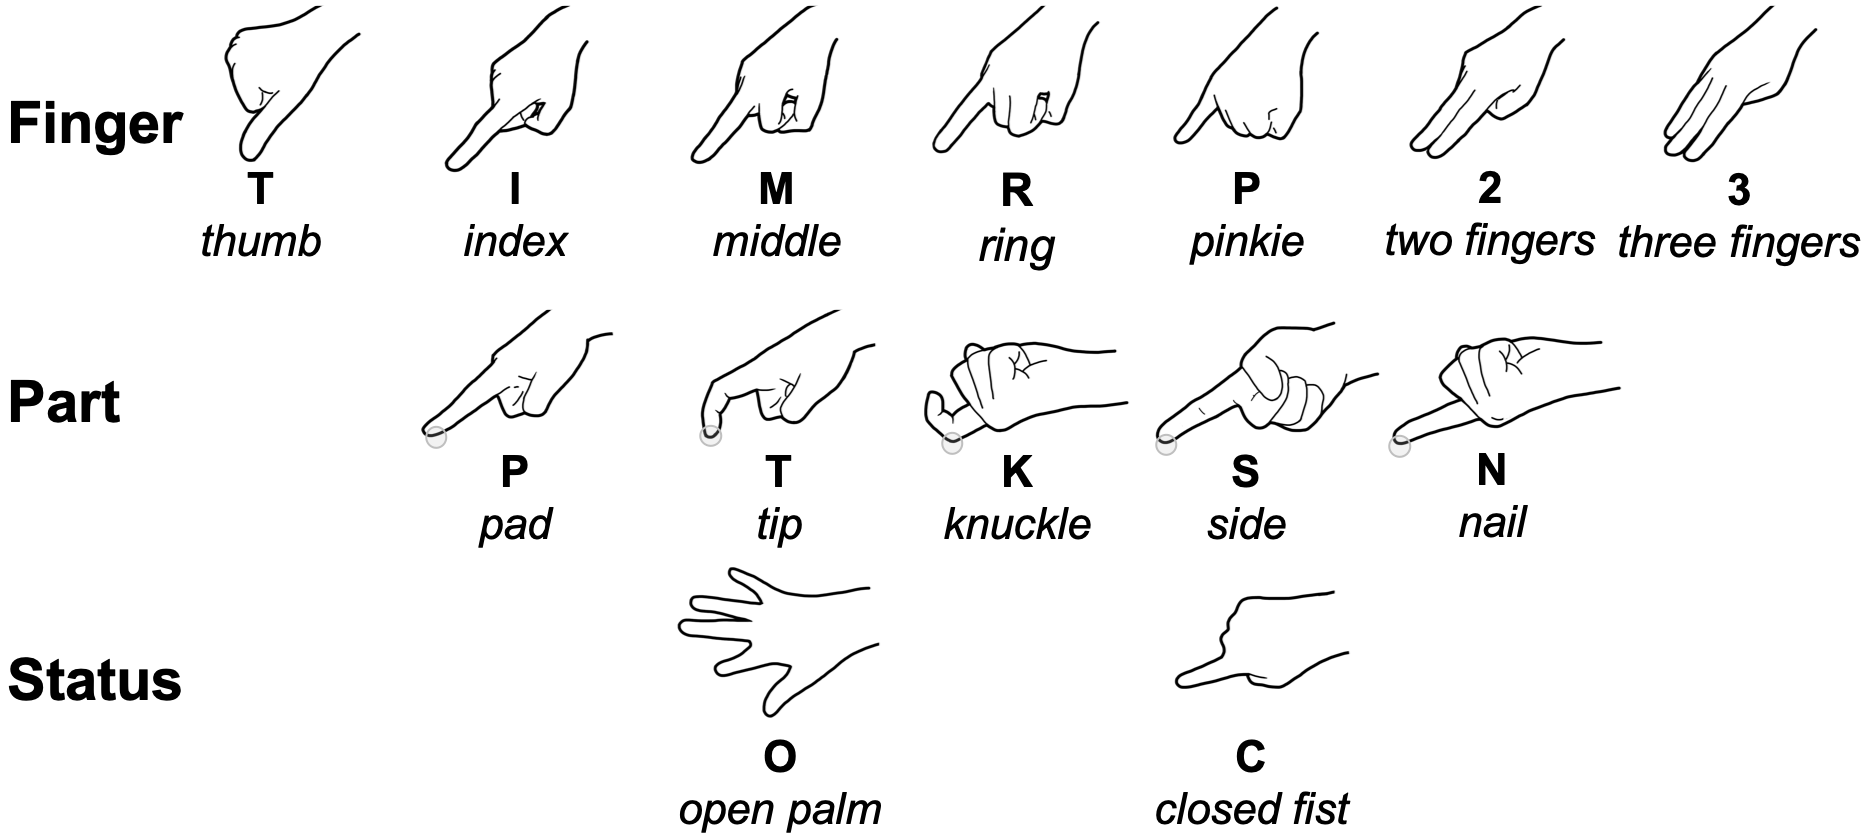
\includegraphics[width=0.8\linewidth]{posture_set.png}
	\caption*{触摸姿态的设计空间有三个维度,分别是哪些手指触摸、手指的哪个部分触摸和手部状态,三个维度的笛卡尔积就是触摸姿态全集。其中,粗体字母是根据每个状态的英文描述起的缩写。}
	\caption{触摸姿态的三维设计空间}
	\label{fig:posture_set}
\end{figure}

以上设计空间中三个维度的笛卡尔积即为触摸姿态的全集,共包含$7\times5\times2=70$种触摸姿态。实验者为他们定义了缩写,例如,五指张开状态下食指指腹触摸的缩写为IPO,其中I对于食指,P对应指腹,O对应五指张开的状态。

\subsubsection{实验设计和过程}

实验者从校园中招募了20名被试,其中7名为女性,被试的年龄是18岁到27岁不等,平均年龄为22.0岁。实验在两种交互表面上开展,分别是水平的桌面和垂直的墙面,它们是日常生活中场景的物体表面。实验采用组内实验设计,实验者采用拉丁方平衡被试在两种不同交互表面上的实验顺序。由于触摸姿态全集包含70中触摸姿态,而实验在两种交互表面上开展,每位被试在$70\times2=140$种设置下体验触摸交互,并给出评分。实验问卷采用了七级李克特量表,在三个方面上收集用户对每种触摸姿态的评分:

\begin{itemize}
\item \textbf{舒适度}:以该姿态触摸的物理和心理轻松程度(1 - 不轻松,7 - 非常轻松)。
\item \textbf{易记度}:记住该触摸姿态的难以程度(1 - 不容易,7 - 非常容易)。
\item \textbf{喜好度}:对该触摸姿态的总体喜好程度(1 - 完全不喜欢,7 - 非常喜欢)。
\end{itemize}

在实验的最后,实验者针对以下问题对被试进行了简短的采访:(1)您认为在本实验的触摸姿态全集之外是否有其它可用的触摸姿态?(2)在日常使用中,您愿意记住多少种不同的触摸姿态?

实验中,被试坐在可调节的椅子上,在开始实验前,被试需要调整座椅,让自己以最舒适的姿态进行接下来的实验。对于每一个触摸姿态,实验者都会首先进行示范,然后被试亲自执行该触摸姿态三遍,然后在问卷中对该触摸姿态的舒适度、易记度和喜好度评分。由于李克特量表的主要通过相对数值对比不同的被测量值,每一次触摸之后,被试都可以通过对比来修改之前作出的评分。被试每执行十个触摸姿态,就需要休息五分钟的时间,以避免疲劳。整个实验耗时一个小时。

\subsubsection{实验结果}

\begin{figure}
	\centering
	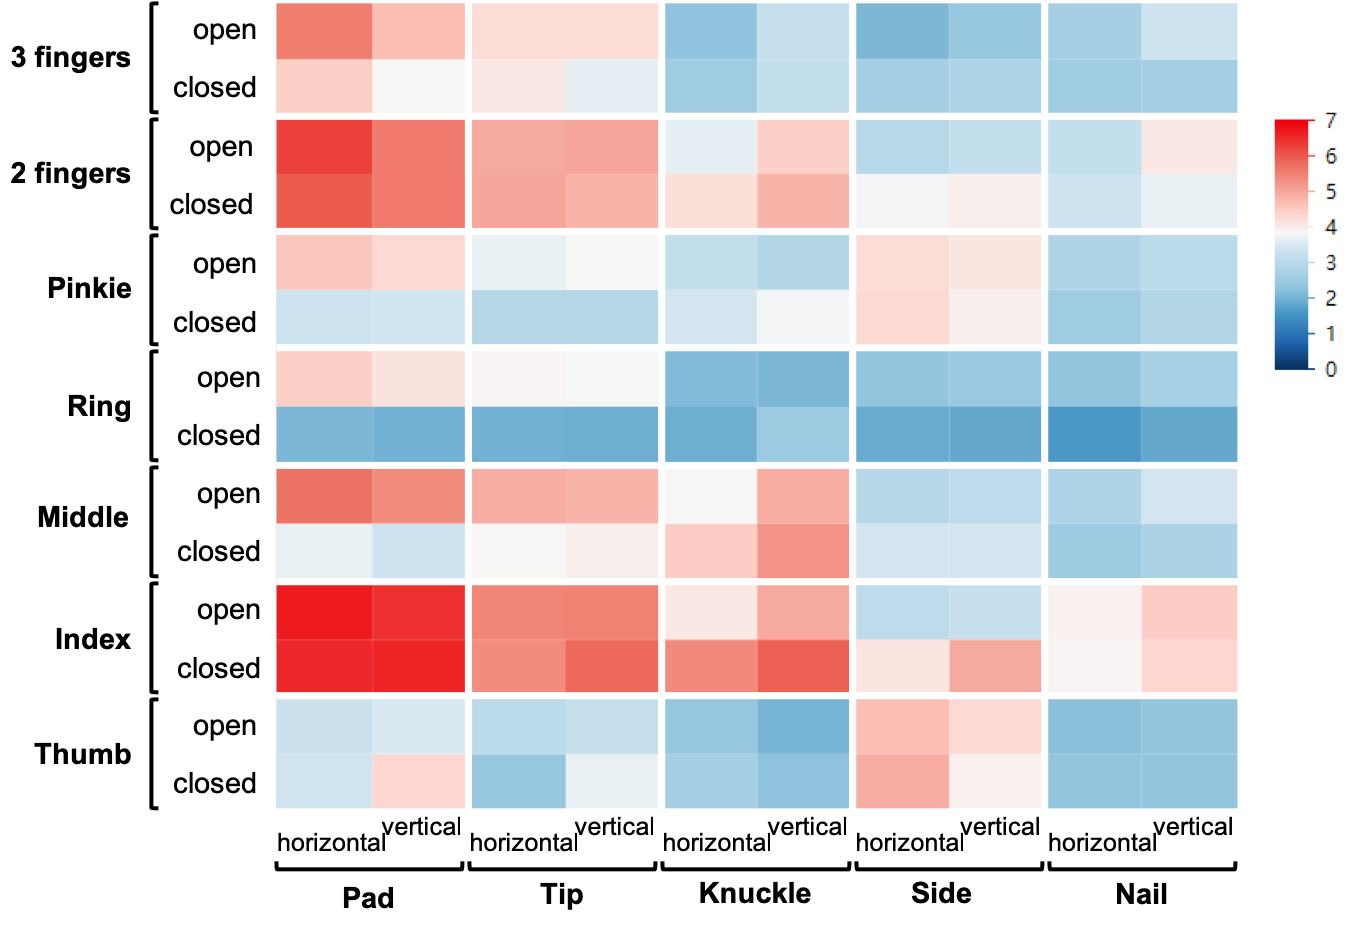
\includegraphics[width=0.8\linewidth]{posture_preference.png}
	\caption*{20名用户对两种交互表面上、70种不同触摸姿态的平均喜好程度,其中,1分表示完全不喜欢,7分表示非常喜欢。}
	\caption{触摸姿态主观评分热力图}
	\label{fig:posture_preference}
\end{figure}

图\ref{fig:posture_preference}展示了被试在水平和垂直交互表面下对所有70种触摸姿态的喜好程度评分,图\ref{fig:posture_top10}展示了被试们最喜好的触摸姿态前十名。Friedman检验显示交互表面的水平和垂直与否并不显著影响用户对各触摸姿态的喜好。在实验后的采访中,没有任何被试报告在触摸姿态全集以外存在其它可用的触摸姿态,因此,实验者认为图\ref{fig:posture_top10}中的就是人们最喜好的十种触摸姿态。

\begin{figure}
	\centering
	
\includegraphics[width=0.8\linewidth]{posture_top10.png}
	\caption*{在人们最喜好的十种触摸姿态中,有七种姿态来自常用的单指或多指指腹点击,另有ITO(食指指尖敲击-张手)、ITC(食指指尖敲击-握拳)和IKC(食指第二关节叩击-握拳)。}
	\caption{人们最喜好的触摸姿态前十名}
	\label{fig:posture_top10}
\end{figure}

喜好程度排名前五的触摸姿态分别是IPO(食指指腹触摸-张手)、IPC(食指指腹触摸-握拳)、2PO(双指指腹触摸-张手)、2PC(双指指腹触摸-握拳)和ITO(食指指尖敲击-张手),这些姿态都是目前常用的触摸手势。喜好程度排六到十名的触摸姿态是ITC、MPO、IKC、2TO和3PO,其中MPO(中指指腹触摸-张手)和IKC(食指第二关节叩击-握拳)值得关注:若触摸交互技术有能力区分食指指腹触摸和中指指腹触摸,部分用户将愿意让中指触摸表达特定的交互语义;食指第二关节叩击是触摸屏上不常用的触摸姿态,但近年来被华为手机用于触发截屏功能,从本实验结果来看,这一交互方式应会广受用户好评。

Friedman检验显示,“哪些手指触摸交互表面”($\chi^2=767.70, p<.0001$)和“手指的哪个部分触摸交互表面”($\chi^2=423.86, p<.0001$)都对被试的主观评分有显著性影响。被试更喜欢用食指、中指、两指和三指进行触摸交互,不喜欢用拇指、无名指和小指触摸。被试只接受指腹点击、指尖敲击和手指第二关节叩击,厌恶手指侧面点击和手指甲敲击。在实验后的采访中,被试报告说他们平均愿意记住 7.45(SD=2.61)个触摸姿态,这是因为,如果交互系统中表达特定交互意图的手势太多,会给用户带来很大的认知负担。因此,实验者认为这十种最受欢迎的触摸姿态是值得进一步研究的,也值得本章的低延迟触摸检测技术去检测,而这十种触摸姿态以外的情形就不需要更多的关注了。

\subsection{实验一B:指环佩戴位置主观喜好程度调研}

本小节介绍一个简短的用户实验,实验目的是调研用户对指环佩戴位置的主观喜好程度,其中,指环是用于触摸交互的智能指环,而非用于装饰的戒指。如图\ref{fig:ring_positions}(a)所示是实验所评测的九种不同的指环佩戴位置,分别是食指、中指和无名指的第一、二、三指骨。实验中,被试需要将一个嵌入了惯性传感器的指环佩戴在手指的不同位置上,在桌面上以自己喜欢的姿态触摸若干次,然后通过问卷对其体验进行主观评分。问卷采用七级李克特量表(1分 - 最差,7分 - 最好),在三个方面上收集用户对指环佩戴位置的主观看法:

\begin{itemize}
	\item \textbf{舒适度}:在此位置上佩戴指环进行触摸交互的舒服程度。
	\item \textbf{接受度}:在此位置上佩戴指环的社会接受程度,比如,是否会吸引他人不必要的注意。
	\item \textbf{喜好度}:对该指环佩戴位置的总体喜好程度。
\end{itemize}

\begin{figure}
	\centering
	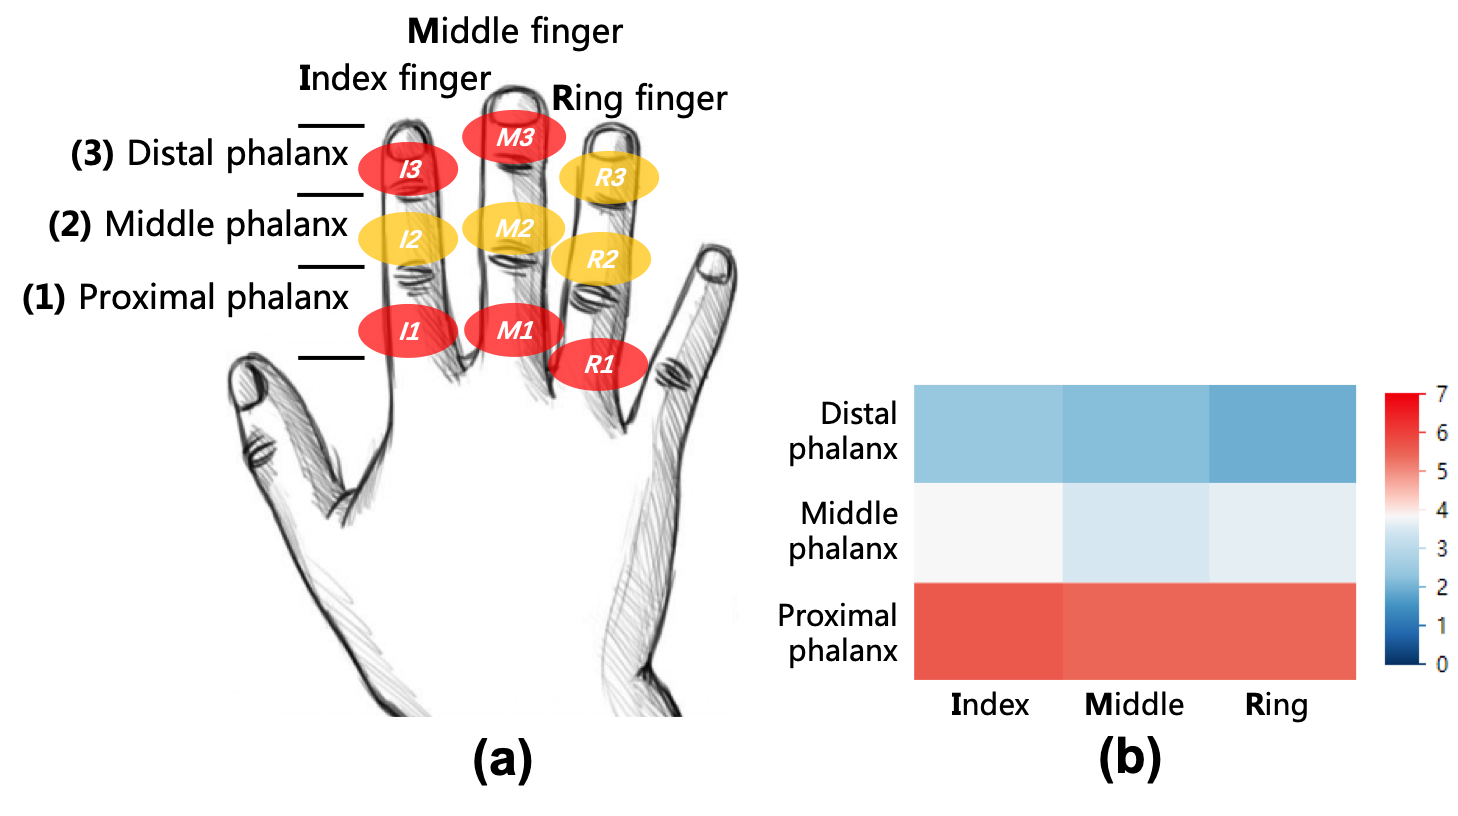
\includegraphics[width=0.8\linewidth]{ring_positions.png}
	\caption*{图a展示了实验所评测的九种不同的指环佩戴位置,实验者为每个位置定义了缩写,例如,I1表示食指的第一指骨;图b是被试对不同指环佩戴位置的喜好程度(1 - 完全不喜欢,7 - 非常喜欢)}
	\caption{指环佩戴位置主观评分热力图}
	\label{fig:ring_positions}
\end{figure}

实验一A的20名被试参与了本实验,如图\ref{fig:ring_positions}(b)所示,被试更喜欢在食指第一指骨(5.65分)、中指第一指骨(5.45分)和无名指第一指骨(5.45分)上佩戴指环,在这些指根的位置上佩戴指环是舒适、且可接受的。将指环佩戴在手指的第二指骨上的主观评分是中肯的,而将指环佩戴在手指末端令人厌恶。实验结果表明,人们更愿意将智能指环佩戴在手指的第一指骨上,但具体是戴在食指、中指还是无名指上都差异不大。因此,基于惯性传感指环的触摸检测技术应尽可能通过指根上的运动传感信号感知触摸事件。

\section{基于机器学习的触摸检测技术}

\subsection{实验二:收集触摸数据}

实验二采集了被试进行触摸交互的惯性传感器数据和头戴式摄像头数据,实验的动机是为两项后续工作提供数据支持:一是基于摄像头的触摸姿态识别,二是基于惯性传感信号的触摸检测技术。

\subsubsection{实验设计和过程}

实验者从校园中招募了12名学生作为被试,其中有4名女性,被试的年龄从20岁到29岁不等,平均年龄为23.1岁。实验分为两大部分,每名被试分别在水平的桌面和垂直的墙面上进行实验。实验采用了组内实验设计,实验者采用拉丁方平衡了水平或垂直表面的实验顺序。

对于每种交互表面,需要进行五段实验:如图\ref{fig:ring_positions}手指上的红色区域所示,每段实验中被试分别在五个不同的位置上佩戴智能指环,这五个位置分别是I1(食指第一指骨)、M1(中指第一指骨)、R1(无名指第一指骨)、I3(食指第三指骨)和M3(中指第三指骨)。选择I1、M1、R1等手指第一指骨位置是因为实验一的结果表明,用户更喜好将智能指环佩戴在这些位置上;而加入I3和M3这两个位置是因为实验者猜测,手指末端上惯性传感器所采样的触摸信号的震动强度更大,利用该信号感知触摸事件的能力可能会更强,实验者需要通过实验对比来验证此猜测是否成立。实验舍弃了采集指环佩戴在I2、M2、R2和R3位置上的触摸数据,这是因为冗余的、时间过长的实验可能会导致被试的疲劳,影响数据的可靠性。

每段实验包含十组,在每组实验中,被试分别以如图\ref{fig:posture_top10}所示的十种触摸姿态接触交互表面,各20次。实验者要求被试尽可能用自然的方式进行触摸交互,每名被试总共进行了$2\times5\times10\times20=2000$次触摸。最后,实验者还收集了一系列空中手势作为负样本,被试将惯性传感指环佩戴在不同的位置,执行画圈、画方框、空中点击等手势。采集空中手势的过程中,被试不允许让手指接触到其它物体。对于每个指环佩戴位置,需要采集持续一分钟的空中手势数据。在实验中,被试要在每200次触摸后休息两分钟,以避免疲劳问题。整个实验持续了一个半小时。

\subsubsection{实验设备}

如图\ref{fig:tapping_ring_config}所示是实验二的实验设置。被试在手指上佩戴了惯性传感指环,头上戴着一种商用手型追踪摄像头(LeapMotion),被试在一块自制的超低延迟触摸板上进行触摸交互。实验通过指环中的惯性传感单元采集加速度和角速度信号,通过LeapMotion采集手部的骨骼点数据,通过触摸板采集接触与否的真值。

\begin{figure}
	\centering
	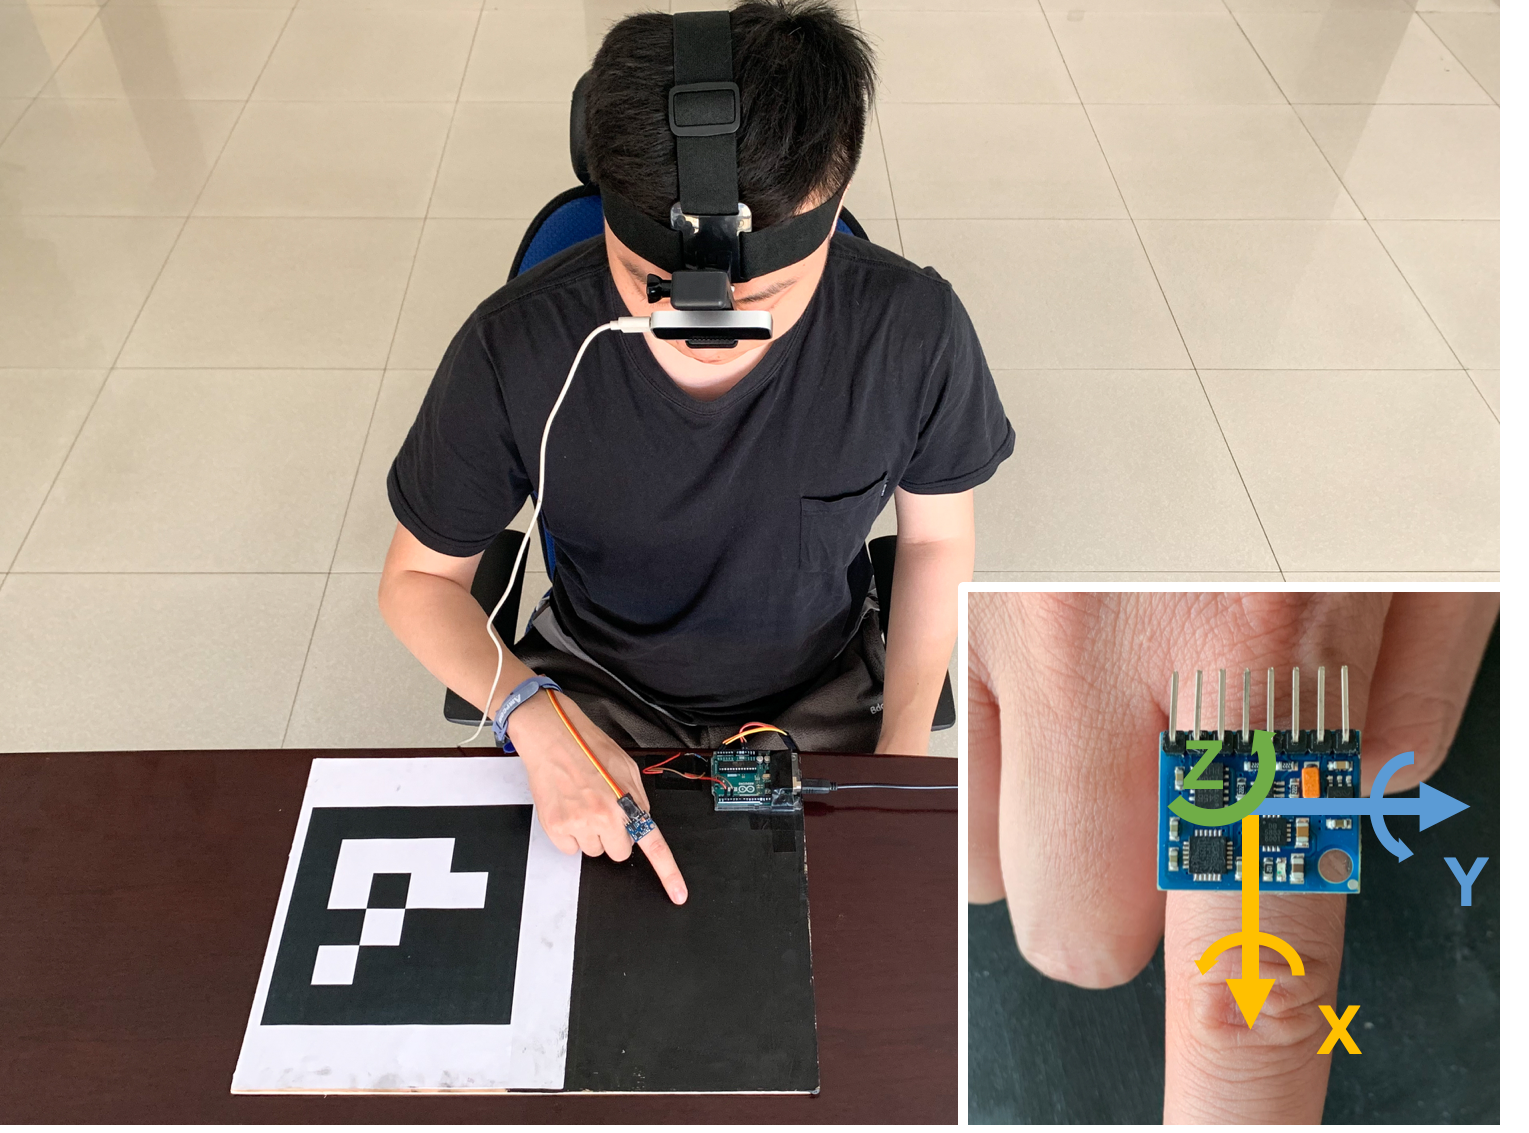
\includegraphics[width=0.6\linewidth]{tapping_ring_config.png}
	\caption*{实验二的实验设置,被试佩戴惯性传感指环接触触摸屏。子图展示了惯性传感指环及其信号所在的坐标系。}
	\caption{实验设置}
	\label{fig:tapping_ring_config}
\end{figure}

惯性传感指环由一个九轴的惯性传感单元(GY-85)和常规的戒指粘合而成,实验者一共制作了四个大小不一的惯性传感指环,以适应不同被试的手指大小,惯性传感单元通过杜邦线连接在Arduino(Uno R3)开发板上。实验者用魔术贴将杜邦线固定在被试的手腕上,以求在最大程度上减轻杜邦线对用户触摸交互造成的影响。超低延迟触摸板是一块覆盖有导电墨水的木板,当手指触摸到木板时,木板与用户的手指形成耦合电容,电容会增加,实验者利用这一现象来判断手指接触木板的精确时间\cite{badger2018capacitive}。

触摸板也通过杜邦线与Arduino连接,它和惯性传感指环共享相同的时间戳,他们的频率都为200赫兹。高速摄像头的图像分析表明,从人触摸木板到Arduino开发版上的信号灯亮起所需时间不超过5毫秒,也就是触摸板的延迟在5毫秒以下。触摸板旁边是一个二维码标识符,用于准确标记交互表面所在位置,以配合LeapMotion计算人的手指上每个关节与交互表面之间的距离。LeapMotion的传感频率为60赫兹,其与Arduino之间的传输延迟大概为20毫秒。LeapMotion在工作原理上依赖其自带的红外照明,一般而言,它时而会出现手型估计失败的情况,为此实验者非常注重实验的关照条件:实验在灯光明亮且避免阳光的环境中进行,触摸板上的导电墨水也专门采用吸收红外光的墨水,为摄像头提供了黑色背景,以上实验环境使得LeapMotion的传感精度得到保障。

\subsubsection{实验数据统计}

本实验共采集了$12\times2000=24000$次触摸的实验数据。实验者开发了一个交互式程序,用以人工剔除明显错误的数据,例如,有时候指甲太长的用户接触触摸板时,触摸板无法及时报告触摸事件。在剔除错误数据之后,实验共产生了超过23900 份有效的数据作为触摸的正样本,实验者从空中手势中随机抽取负样本,正样本和负样本的数量相同。

\subsection{基于机器学习的触摸姿态分类}

本小节将介绍基于支持向量机(SVM)的触摸姿态分类方法,该方法较为直观,其目的只是评测采用视觉方法分类触摸姿态的可行性,而非本文的贡献。若该方法的分类准确率达到可观的水平,说明本章提出的MR头盔加智能指环的组合不仅可以检测触摸事件,还能区分不同的触摸姿态。

\subsubsection{技术方案}

本小节参考了相关论文\cite{de2016skeleton}提取手部骨骼特征,特征包括手指尖与交互平面的距离、手指尖之间的距离、手指尖与手掌的距离和手指尖与手掌平面之间的夹角,这些值拼接成19维的手型特征向量,实验者根据此特征向量提取方法训练SVM模型,该模型即可分类不同的触摸姿态。

\subsubsection{评测结果}

如表\ref{tab:posture_accuracy}所示,实验者采用留一(被试)交叉验证法评估触摸姿态分类的准确率。IPO、IPC、2PC、IKC这四种最常用的触摸姿态的四分类准确率达到99.0\%,这说明触摸姿态四分类具有较高的可行性;在四分类的基础上,外加2PO、MPO 和 3PO这三种触摸姿态,得到七分类的准确率为88.5\%,这说明触摸姿态七分类的准确率仍在可接受范围内;然而,所有常用触摸姿态的十分类准确率却很不理想,准确率仅为77.0\%,这说明就目前的视觉技术而言,要准确分类十个或者以上的触摸姿态仍比较困难。

\begin{table}
	\centering
	\caption{触摸姿态分类的准确率(括号中数值为标准差)}
	\begin{tabular}{llll}
		\toprule
		无 & 四分类 & 七分类  & 十分类 \\
		\midrule
		水平桌面 & 99.1\% (1.3\%) & 89.5\% (3.9\%) & 76.4\% (6.8\%) \\
		垂直墙面 & 99.0\% (1.4\%) & 87.6\% (4.8\%) & 77.6\% (6.7\%) \\
		\bottomrule
	\end{tabular}
	\label{tab:posture_accuracy}
\end{table}

上述实验结果表明,头戴式前置摄像头大约可以稳健地区分四到七种不同的触摸姿态。随着手部跟踪技术的发展\cite{ge2018hand, spurr2018cross, yuan2018depth},作者认为,通过触摸姿态的多样化来丰富触摸交互将很快成为可能。

\subsection{基于机器学习的触摸检测技术}

本小节将介绍基于支持向量机(SVM)的触摸检测技术。支持向量机是一种简单的机器学习方法,具有开发敏捷的特点,因此,本小节的目的并不是实现终版触摸检测技术,而是通过简单的机器学习方法探索指环触摸检测技术中尚待确定的因素。

\subsubsection{数据分析}

惯性传感指环的中能收集到的数据包括指环的加速度、角速度和磁力计数据。由于磁力计数据的刷新频率只有8赫兹,实验者舍弃了磁力计数据。原始的加速度数据中混杂了重力,实验者通过Madgwick过滤器\cite{madgwick2010efficient}将原始加速度信号分解为加速度和重力。最后,经过处理的实验数据共包含九个维度,包括三轴加速度、三轴角速度和三轴重力。

\begin{figure}
	\centering
	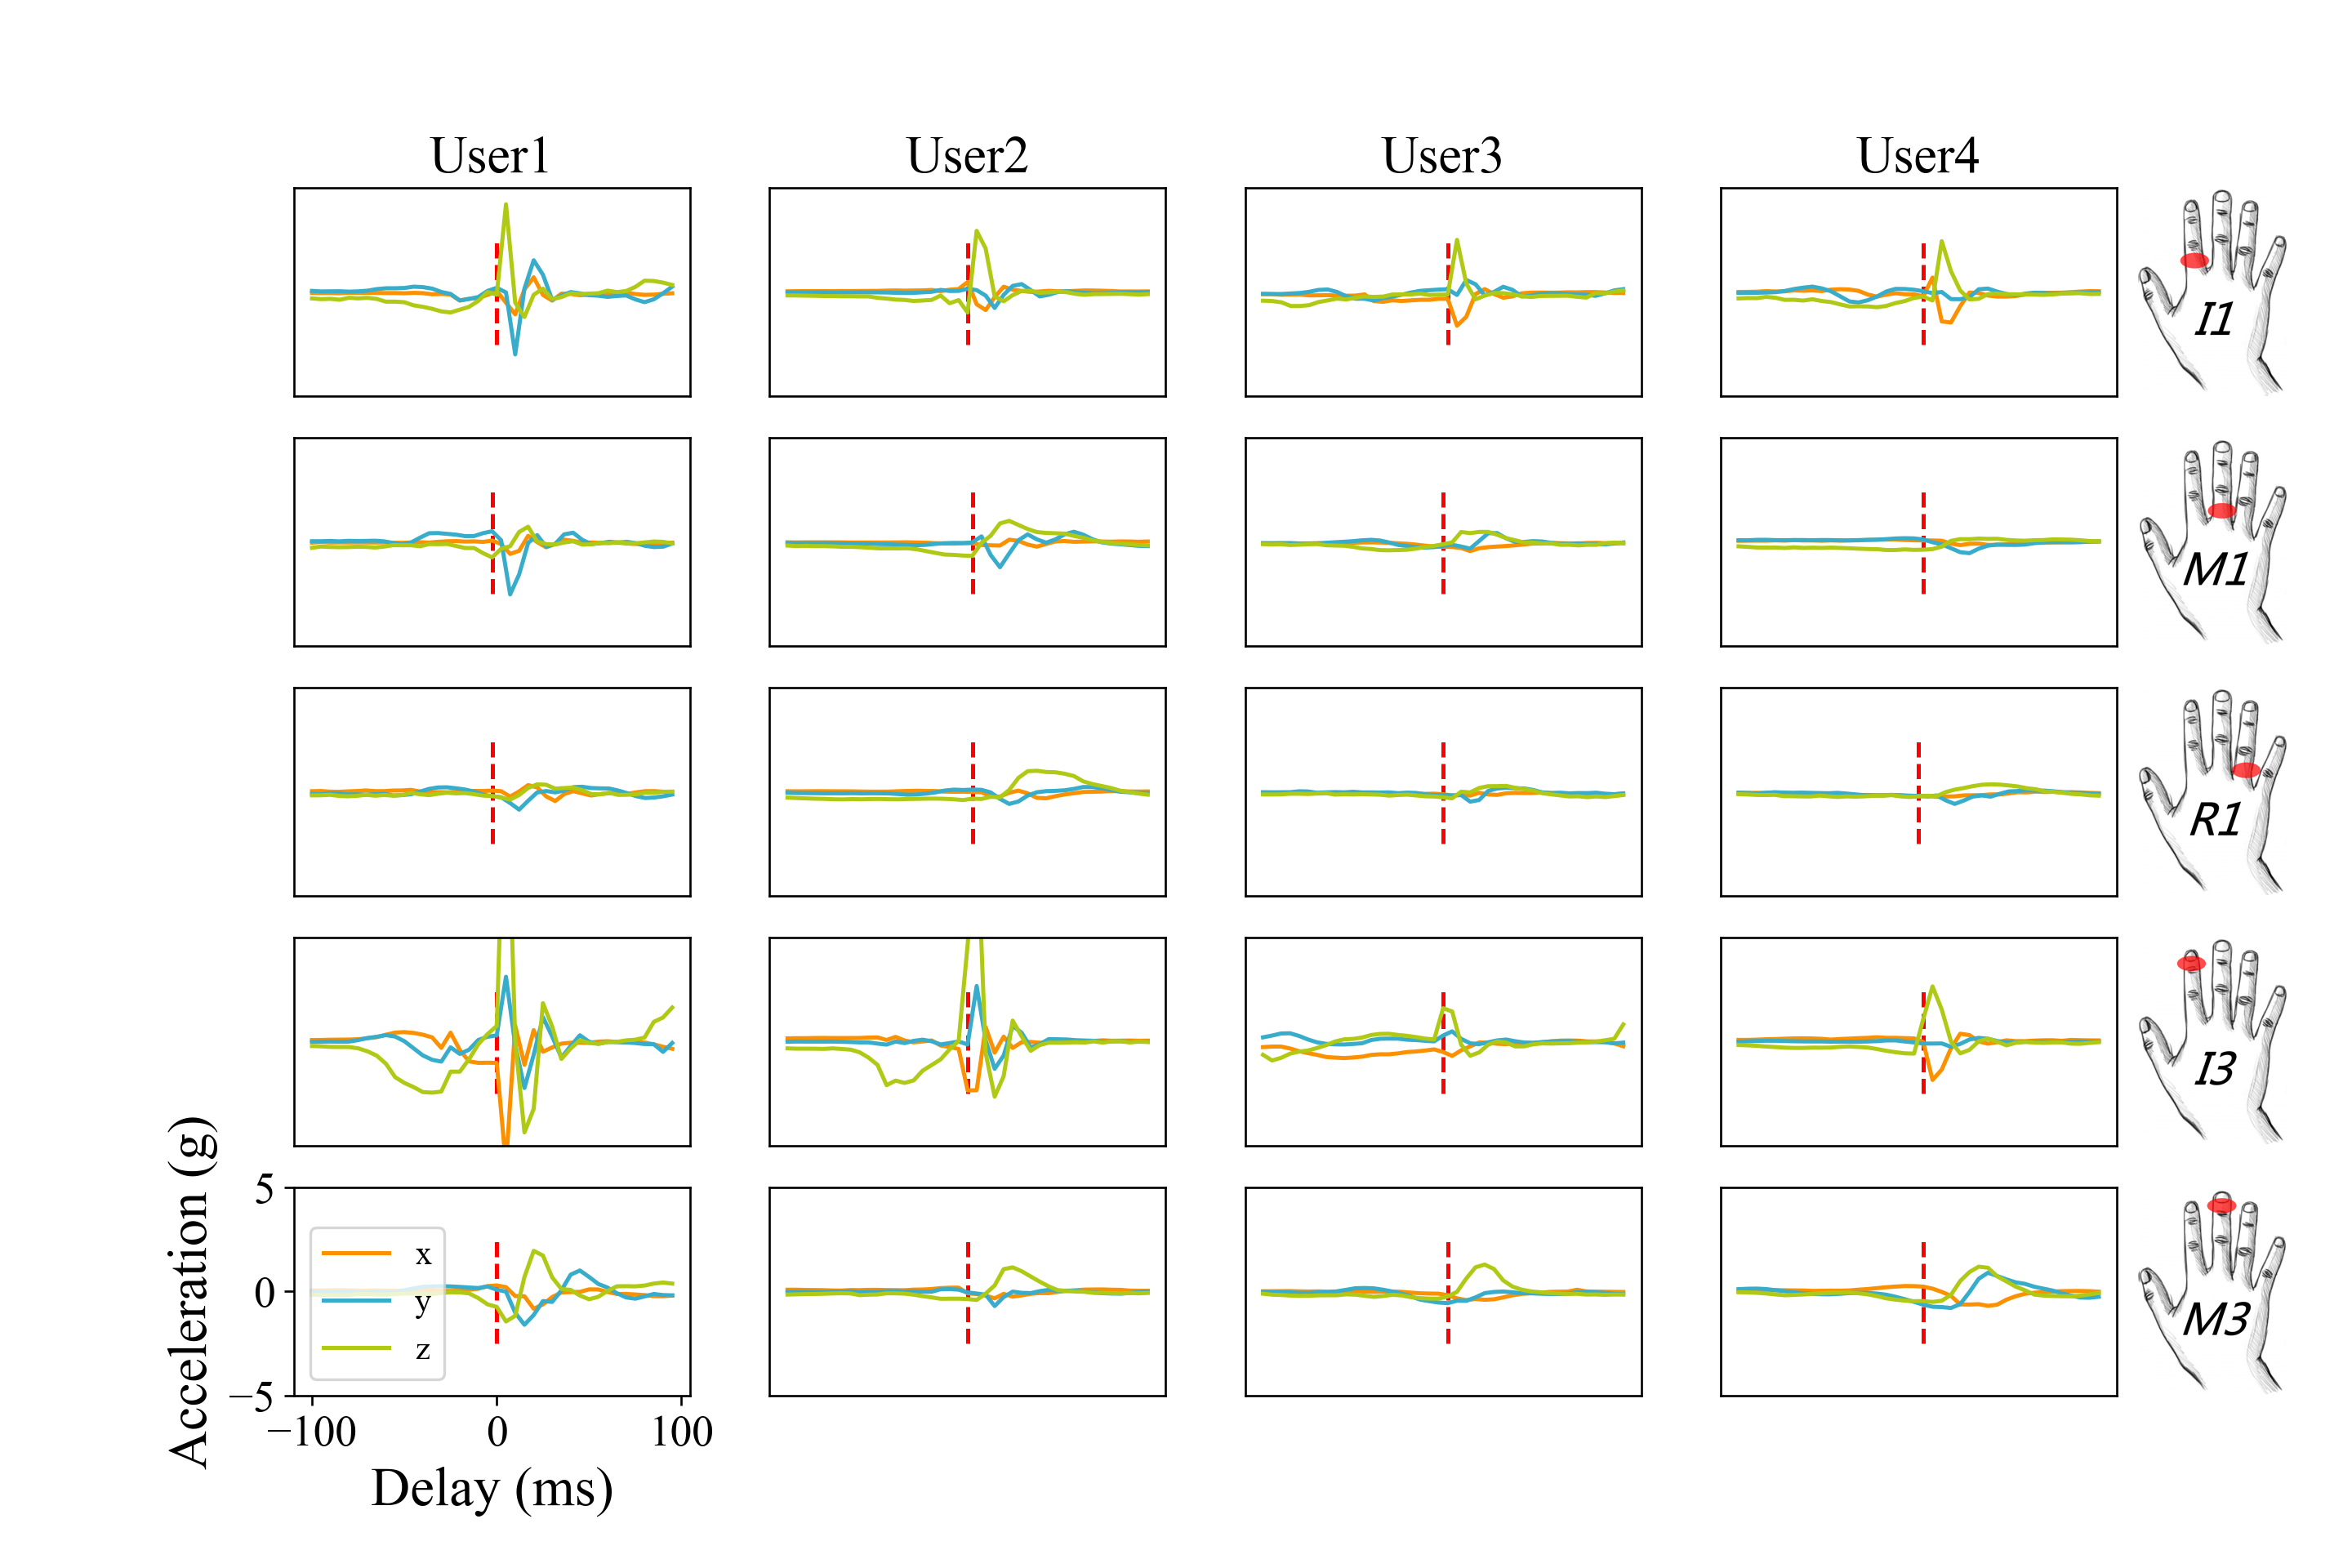
\includegraphics[width=0.8\linewidth]{IMU_acc_hands.png}
	\caption*{图中展示了被试执行食指指腹触摸时的惯性传感器加速度信号,四纵列子图对应四个不同的被试,五横列子图对应了五种不同的指环佩戴位置。}
	\caption{加速度信号图示}
	\label{fig:IMU_acc_hands}
\end{figure}

如图\ref{fig:IMU_acc_hands}所示,本小节以食指指腹点击这一触摸姿态为例分析数据规律。从图中可以看出,触摸导致的震动会传导到各个手指的各个位置上,形成一个幅度较大、较为尖锐的波峰。当指环佩戴在引发触摸的手指上时(如食指第一指骨、食指第三指骨),震动带来的波峰会在触摸后10毫秒内达到峰值;当指环佩戴在其它手指上时,震动带来的波峰则会在20毫米内达到峰值。对于特定的指环佩戴位置,不同被试数据中的加速度波形是类似的。通过观察波形图,实验者推断,触摸发生前后加速度的最大值、最小值、平均值、偏度和峰度等多种特征都可能有助于对触摸的感知。

\begin{figure}
	\centering
	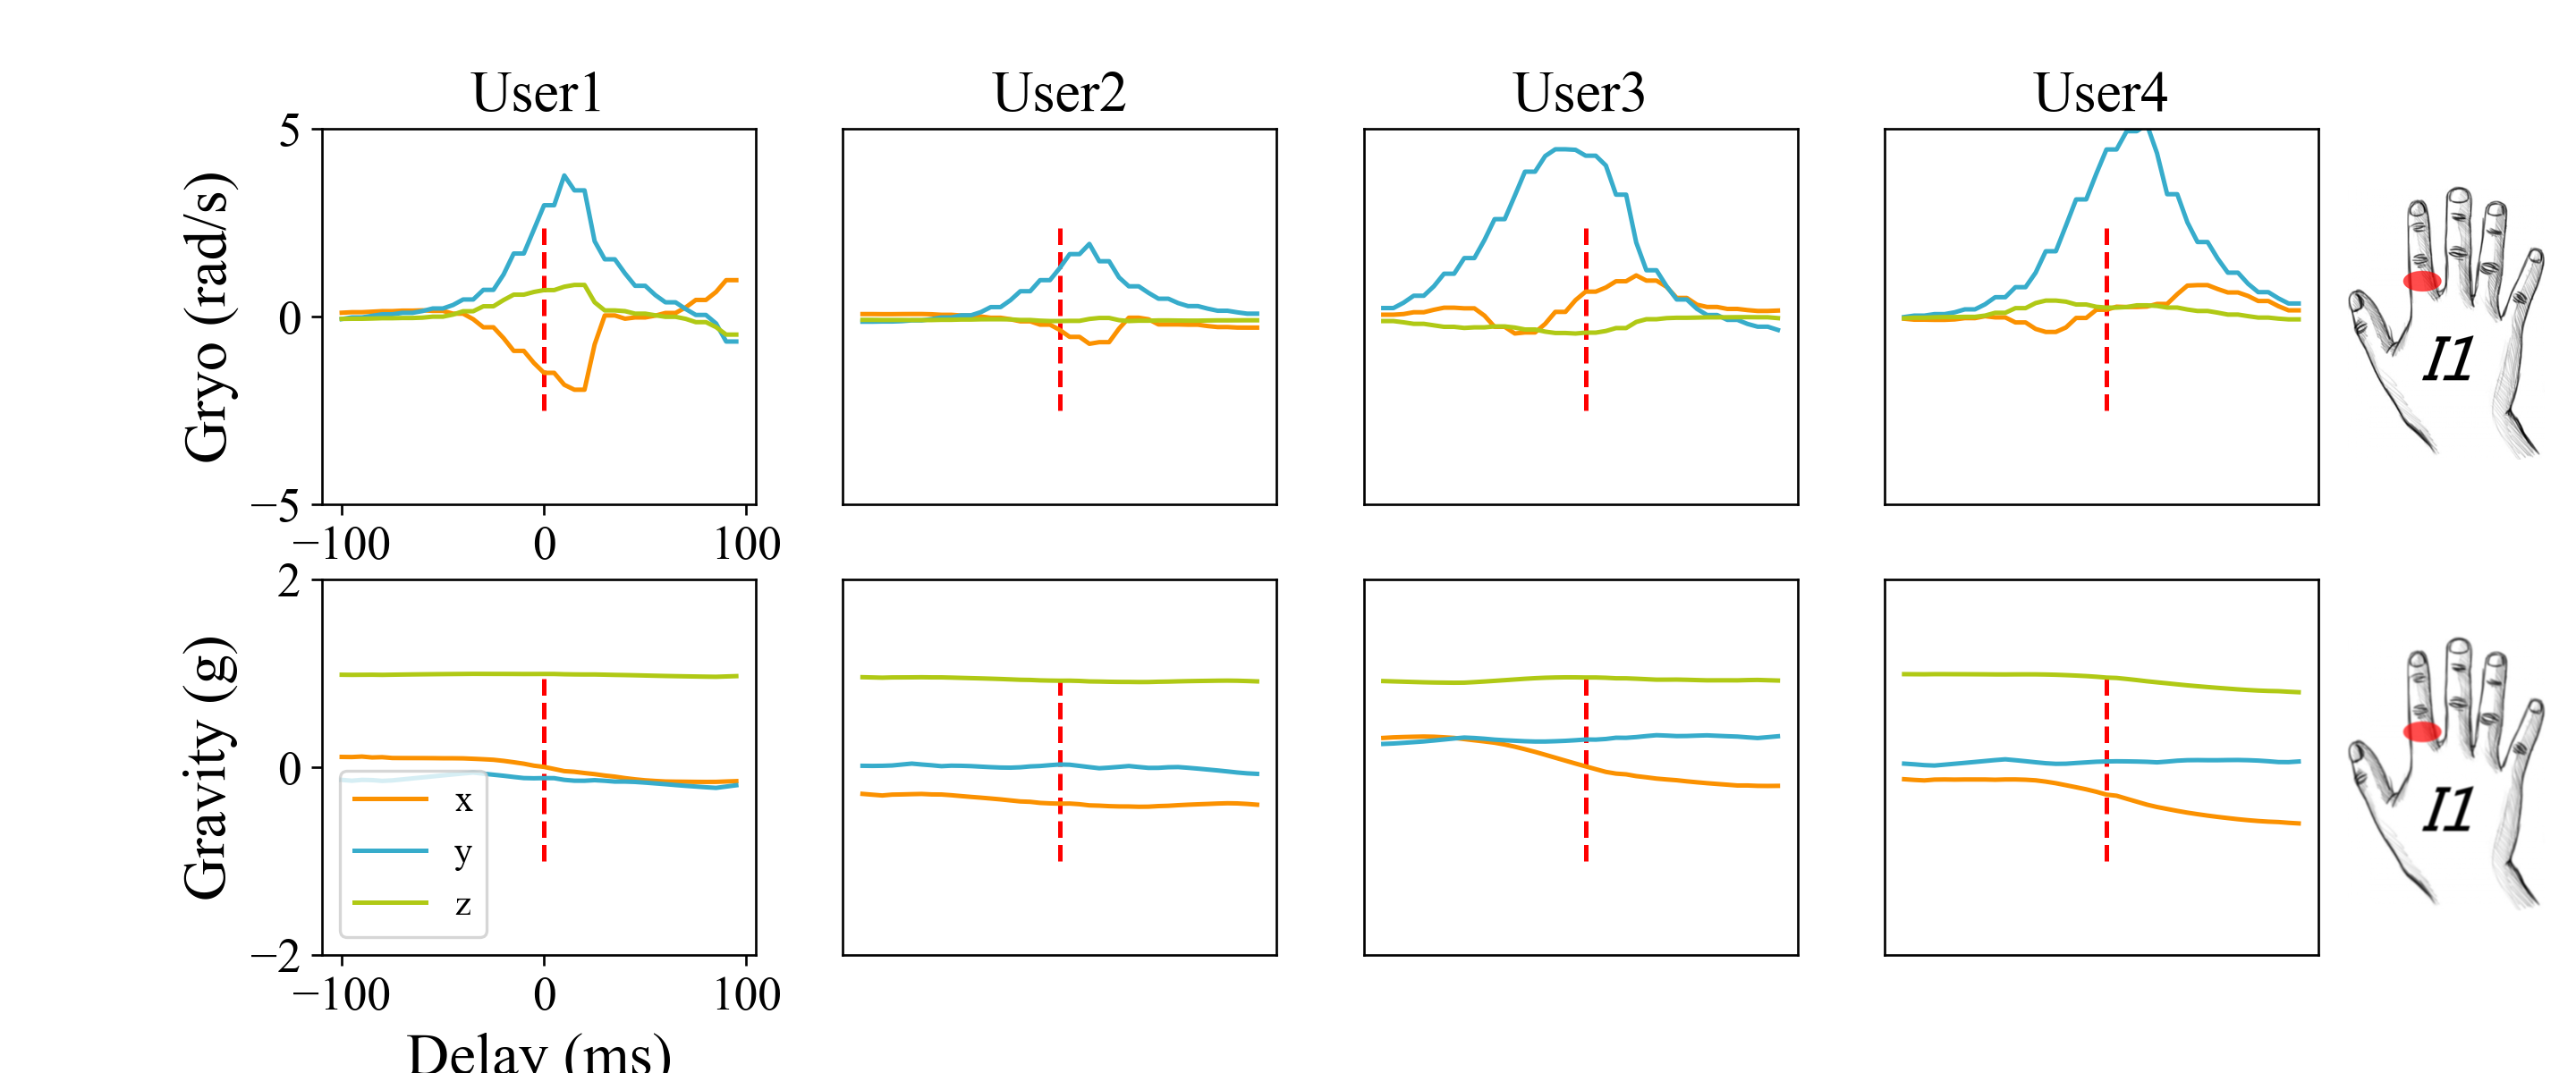
\includegraphics[width=0.8\linewidth]{IMU_gyr_hands.png}
	\caption*{图中展示了被试执行食指指腹触摸时惯性传感器的角速度和重力信号,其中惯性传感指环佩戴在食指第一指骨上,四纵列子图对应四个不同的被试。}
	\caption{角速度和重力信号图示}
	\label{fig:IMU_gyr_hands}
\end{figure}

如图\ref{fig:IMU_gyr_hands}所示是角速度和重力的波形。在触摸发生前后,角速度和重力变化也是有规律的,例如,由于触摸交互时人的手掌大致平行于交互表面,所以所有被试的重力数据都是相似的,若有一段手部运动的重力数据波形与图中所示的形态不符,说明它更有可能属于空中手势交互,而不是触摸交互。上述观察表明,来自惯性传感指环的可用信息是非常丰富的,若利用机器学习方法综合考虑各方面的有效信息,应能在触摸检测的性能上超越先前工作中的阈值方法\cite{lam2002mids, oh2017anywheretouch, niikura2014anywhere}。

\subsubsection{触摸检测分类器}

触摸检测分类器是根据一段时间内惯性传感信号,判断此刻是否发生触摸事件的二分类模型,是基于机器学习的触摸检测技术的核心。分类器从十帧(50毫秒)的传感信号中提取特征,对于九轴惯性传感器数据中的每一个维度,分类器计算其最大值、最小值、均值、偏度和峰度,然后将这些值拼接成45维的数组,作为机器学习模型的特征向量。

\begin{figure}
	\centering
	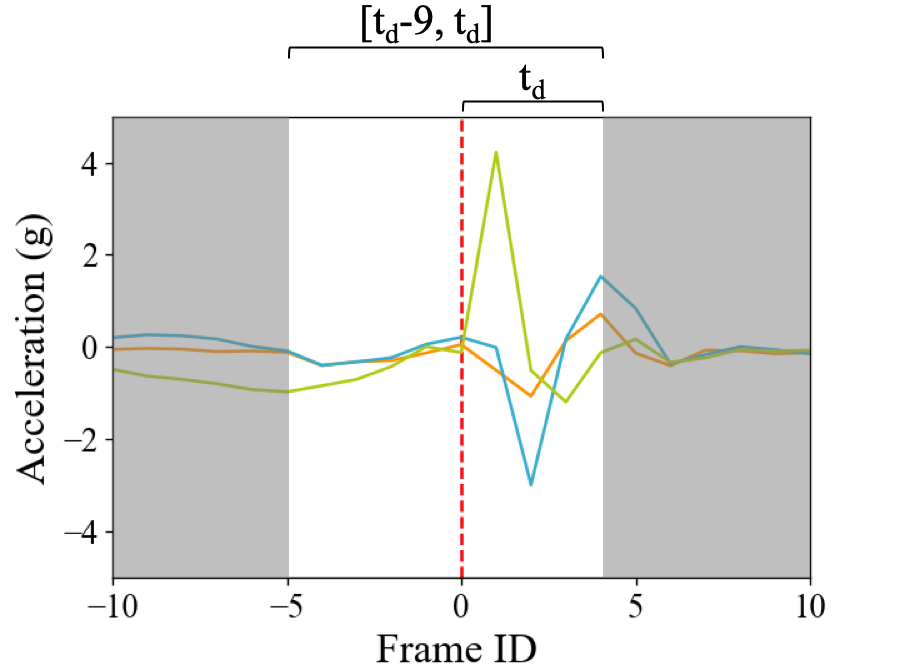
\includegraphics[width=0.8\linewidth]{tapping_ring_classifier.png}
	\caption*{触摸检测分类器是判断当前时刻是否发生触摸事件的二分类模型,其原理是将十帧(50毫秒)的传感信号提取成特征向量,而后使用支持向量机训练得模型。}
	\caption{触摸检测分类器}
	\label{fig:tapping_ring_classifier}
\end{figure}

如何选择信号采样的时间窗口,是一个值得探讨的问题。触摸导致的震动传输到惯性传感器的位置需要一定的时间,如果在震动抵达惯性传感器之前就贸然判定触摸事件是否发生,准确率会受到很大的影响。因此,在本小节所介绍的触摸检测技术中,检测延迟并不是越低越好,检测延迟和准确率是此消彼长的权衡惯性,实验者必须通过模拟实验来确定延迟的最佳取值。如图\ref{fig:tapping_ring_classifier}所示,本小节将$t_d(0<t_d<10)$定义为触摸检测分类器的延迟,设触摸发生在第0帧,则分类器由时间窗口$[t_d-9,t_d]$的信号所提取的特征训练而得。$t_d$的值的选取是一个值得权衡的问题,$t_d$的值越大,分类器就越能够利用触摸实际发生后的震动信号,分类的准确率将会提高,但与此同时检测的延迟也会增加。因此,实验者必须通过测试来给模型选定合适的延迟$t_d$。若给定$t_d$,分类器的训练过程如下:从时间窗口$[t_d-9,t_d]$的惯性传感信号中提取特征作为正样本;为了避免提前汇报触摸事件,需从时间窗口$[-14,-5]$的惯性传感信号中提取特征作为负样本;此外,需要从空中手势中截取信号,提取特征作为负样本。最后,针对以上正负样本数据集运行支持向量机来训练分类器模型。

\subsubsection{检测延迟优化}

上一小节提到,触摸检测分类器的检测延迟$t_d$是由技术实现者自行决定的,是一个检测准确率和延迟之间权衡的问题:一方面,检测延迟越低,触摸检测的准确率就越低;另一方面,检测延迟过高,又会直接影响用户体验。因此,如图\ref{fig:acc_over_delay}所示,实验者通过实验评测了$t_d$取不同的值时,触摸检测技术的准确率。从图中可以看出,总体上来说更高的检测延迟的确可以提高模型的预测准确率,但是当延迟提高至20毫秒以后,再往上延长检测时间的意义就不大了:混合方差分析表明,在20毫秒以内,模型的延迟$t_d$对模型预测准确率有显著性影响($F_{3,33}=133.4,p<.0001$);在20毫秒以后,图中的曲线就开始收敛了($F_{2,22}=0.011,p=.99$)。这说明,触摸检测分类器的检测延迟$t_d$应设置为20毫秒,既能支持较高的检测准确率(99.3\%),又能避免用户察觉到延迟的存在。

\begin{figure}
	\centering
	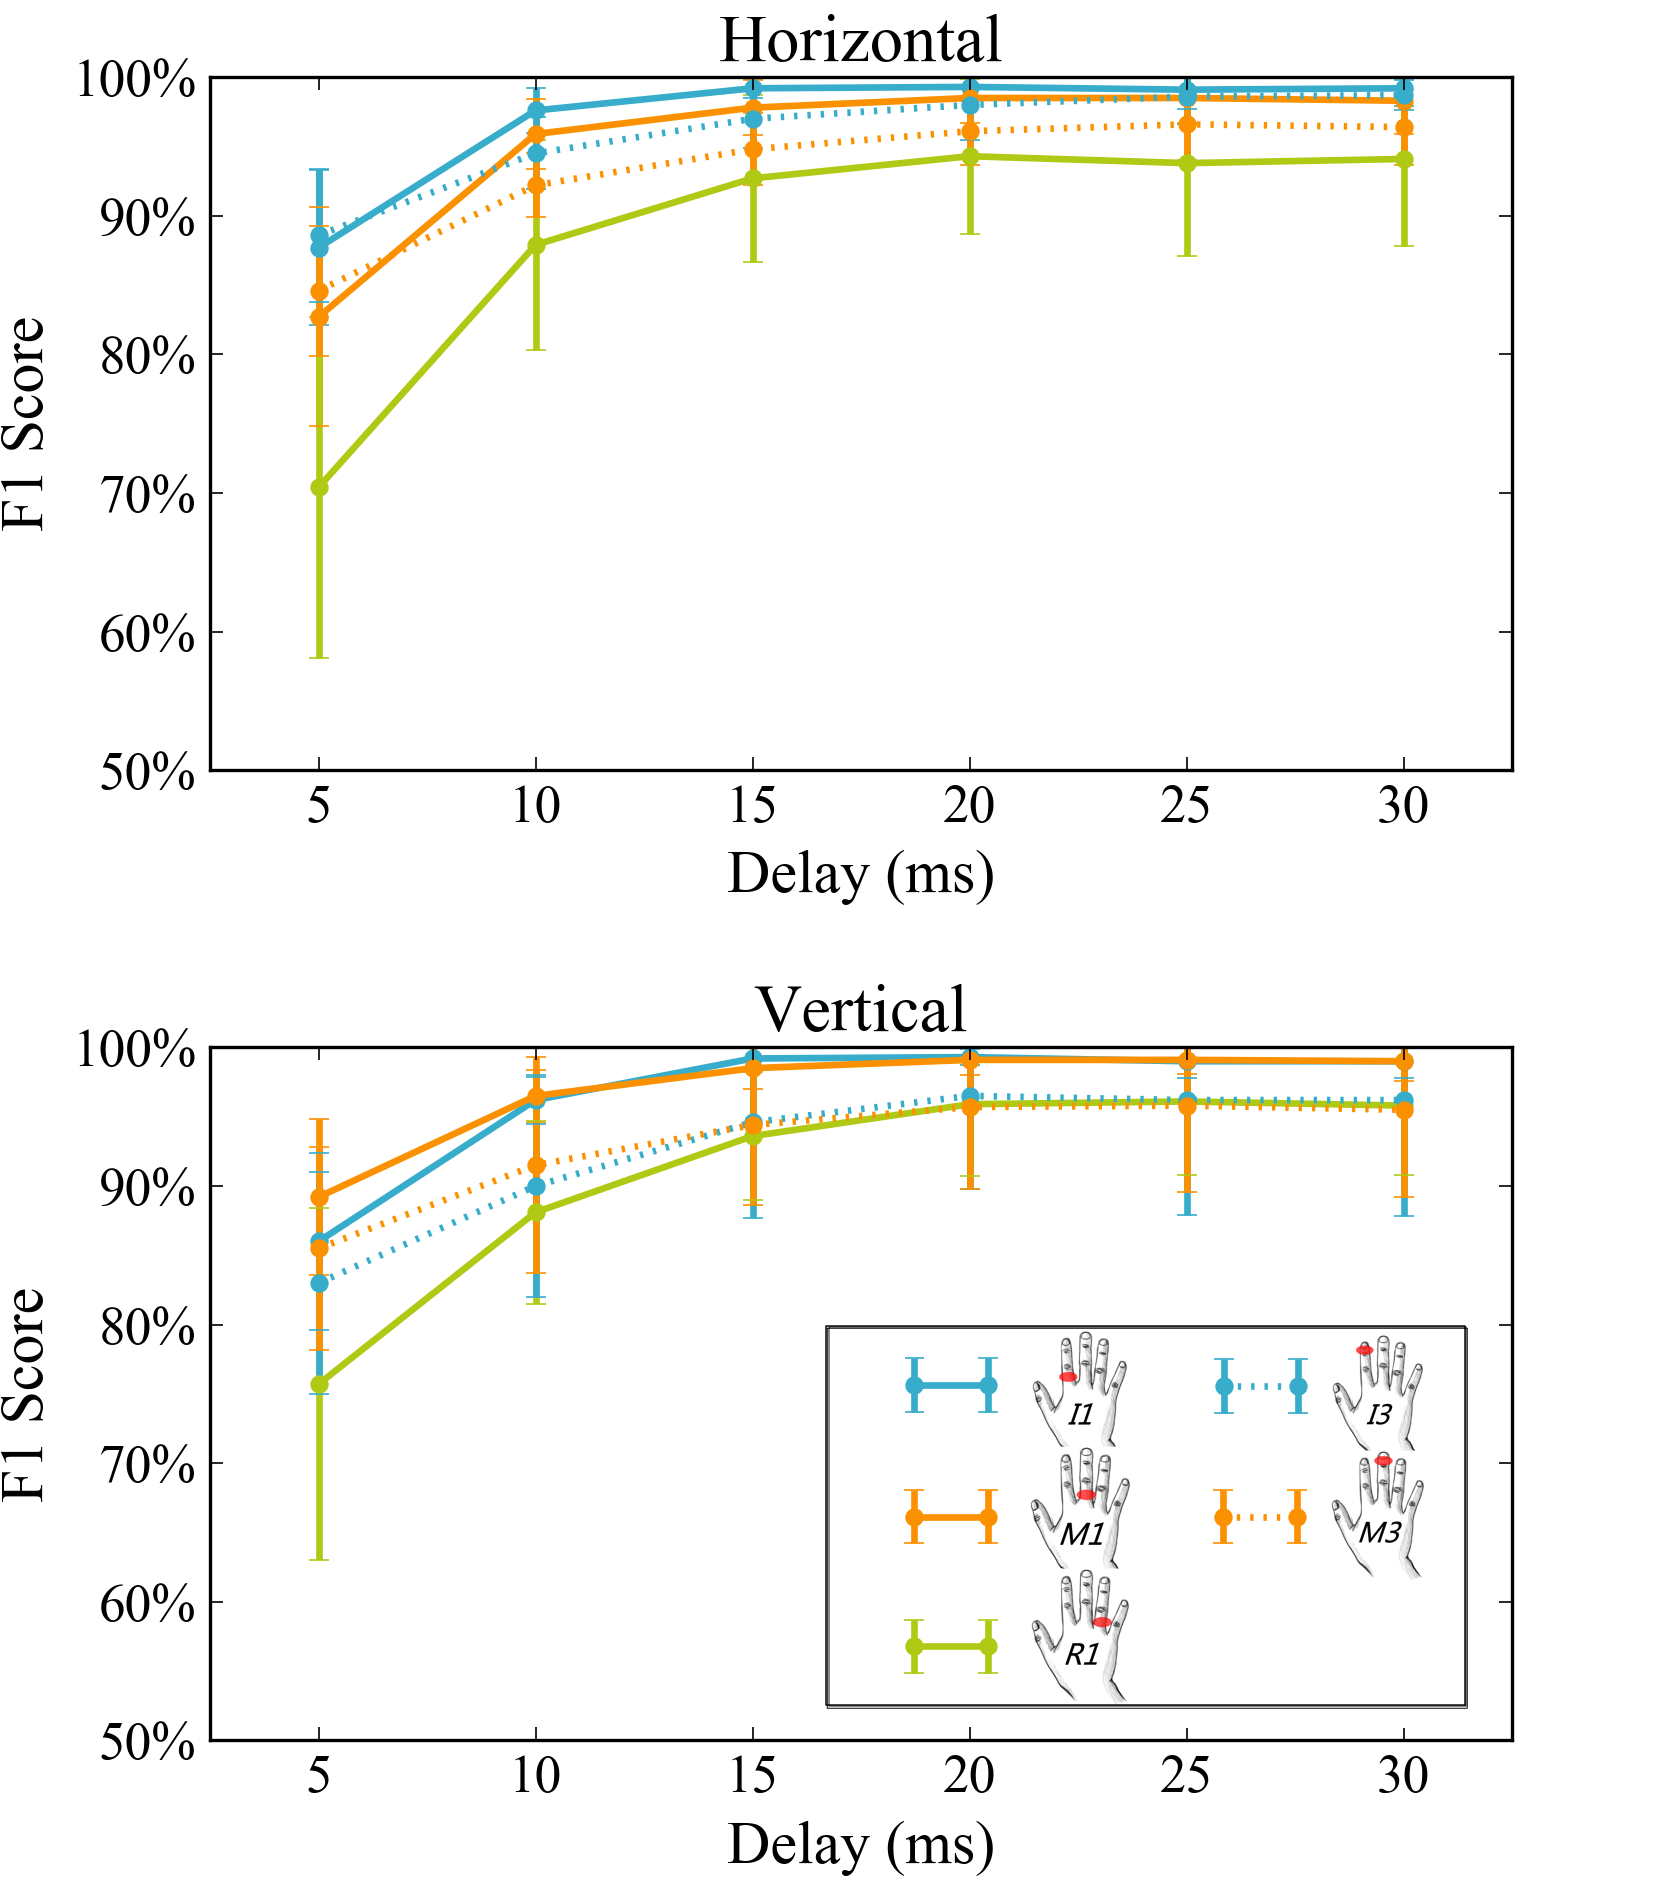
\includegraphics[width=0.8\linewidth]{acc_over_delay.png}
	\caption*{在本小节所介绍的触摸检测技术中,检测准确率和延迟之间是一个此消彼长的权衡问题,图中展示了指环佩戴在不同位置上时,检测准确率和延迟之间的关系。}
	\caption{触摸检测准确率与延迟之间的关系}
	\label{fig:acc_over_delay}
\end{figure}

\subsubsection{指环佩戴位置对比}

\begin{table}[!htbp]
	\centering
	\begin{tabular}{ll|l|l|l|l|l}
		\toprule
		& 指环位置 & I1               & M1            & R1            & I3             & M3            \\
		\midrule
		\multirow{3}{*}{水平} & 精准率 & 99.7\%(0.5\%) & 99.2\%(1.0\%) & 97.6\%(1.9\%) & 99.1\%(1.3\%)  & 98.3\%(1.4\%) \\
		& 召回率    & 98.9\%(1.6\%)    & 97.9\%(3.0\%) & 91.7\%(9.2\%) & 97.1\%(4.4\%)  & 94.1\%(4.1\%) \\
		& F1分数  & 99.3\%(1.0\%)    & 98.5\%(1.8\%) & 94.3\%(5.6\%) & 98.0\%(2.5\%)  & 96.1\%(2.5\%) \\ \hline
		\multirow{3}{*}{垂直}   & 精准率 & 99.7\%(0.6\%)    & 99.3\%(1.1\%) & 98.1\%(1.5\%) & 98.3\%(2.1\%)  & 98.4\%(1.9\%) \\
		& 召回率    & 99.0\%(0.9\%)    & 98.8\%(1.8\%) & 94.0\%(8.4\%) & 95.4\%(10.8\%) & 93.7\%(9.8\%) \\
		& F1分数  & 99.3\%(0.6\%)    & 99.1\%(1.1\%) & 95.9\%(5.3\%) & 96.5\%(6.7\%)  & 95.7\%(5.9\%) \\
		\bottomrule
	\end{tabular}
	\caption{指环佩戴在不同位置上时的触摸检测准确率(触摸检测延迟为20毫秒)}
	\label{tab:acc_over_placement}
\end{table}

在确定20毫秒的检测延迟效果最佳之后,实验者对比了20毫秒延迟下,指环佩戴在不同位置上的检测准确率。结果如表\ref{tab:acc_over_placement}所示,当指环佩戴在I1(食指第一指骨)上时,触摸检测分类器的性能是最好的,准确率(F1综合评价指标)达到99.3\%;次好的指环佩戴位置是M1(中指第一指骨),准确率为98.8\%。方差分析显示,指环佩戴位置对检测准确率有显著性影响($F_{4,44}=6.45,p<.001$),而交互表面的方向则对检测准确率没有显著影响($F_{1,11}=0.09,p=.76$)。后验检测显示I1指环佩戴位置显著优于R1(p<.001)、I3(p<.005)和M3(p<.005);M1显著优于R1(p<.005)、I3(p<.05)和M3(p<.01)。

实验一曾提到,实验者将指环佩戴位置I3和M3(食指、中指第三指骨)也加入了实验序列,其原因是实验者猜测此处能传感到更强的触摸震动,有利于触摸检测的准确率。然而,从本实验的结果看来,此猜测被证伪了,当指环佩戴在位置I3和M3上时触摸检测的准确率反而降低了。通过观察实验数据,实验者找到了两点原因:首先,虽然位置I3和M3上的惯性传感器能传感到更强的振动,但是其噪声也被放大了;其次,一根手指触摸交互表面所产生的震动不能很好地传递到另一根手指的指尖。

综合本小节实验结果和本章中对指环佩戴位置的主观喜好程度调研,将惯性传感指环佩戴在I1或M1位置(食指或中指第一指骨)上是最佳选择,既能提高指环触摸检测技术的检测准确率,又能满足用户的主观喜好。

\subsubsection{综合评测}

以上结果表明,触摸检测分类器在20毫秒的检测延迟下,在用户将惯性传感指环佩戴在食指第一指骨上时,性能最佳。因此,我们在此最佳设置下对触摸检测分类器做全面的评测。

\begin{figure}
	\centering
	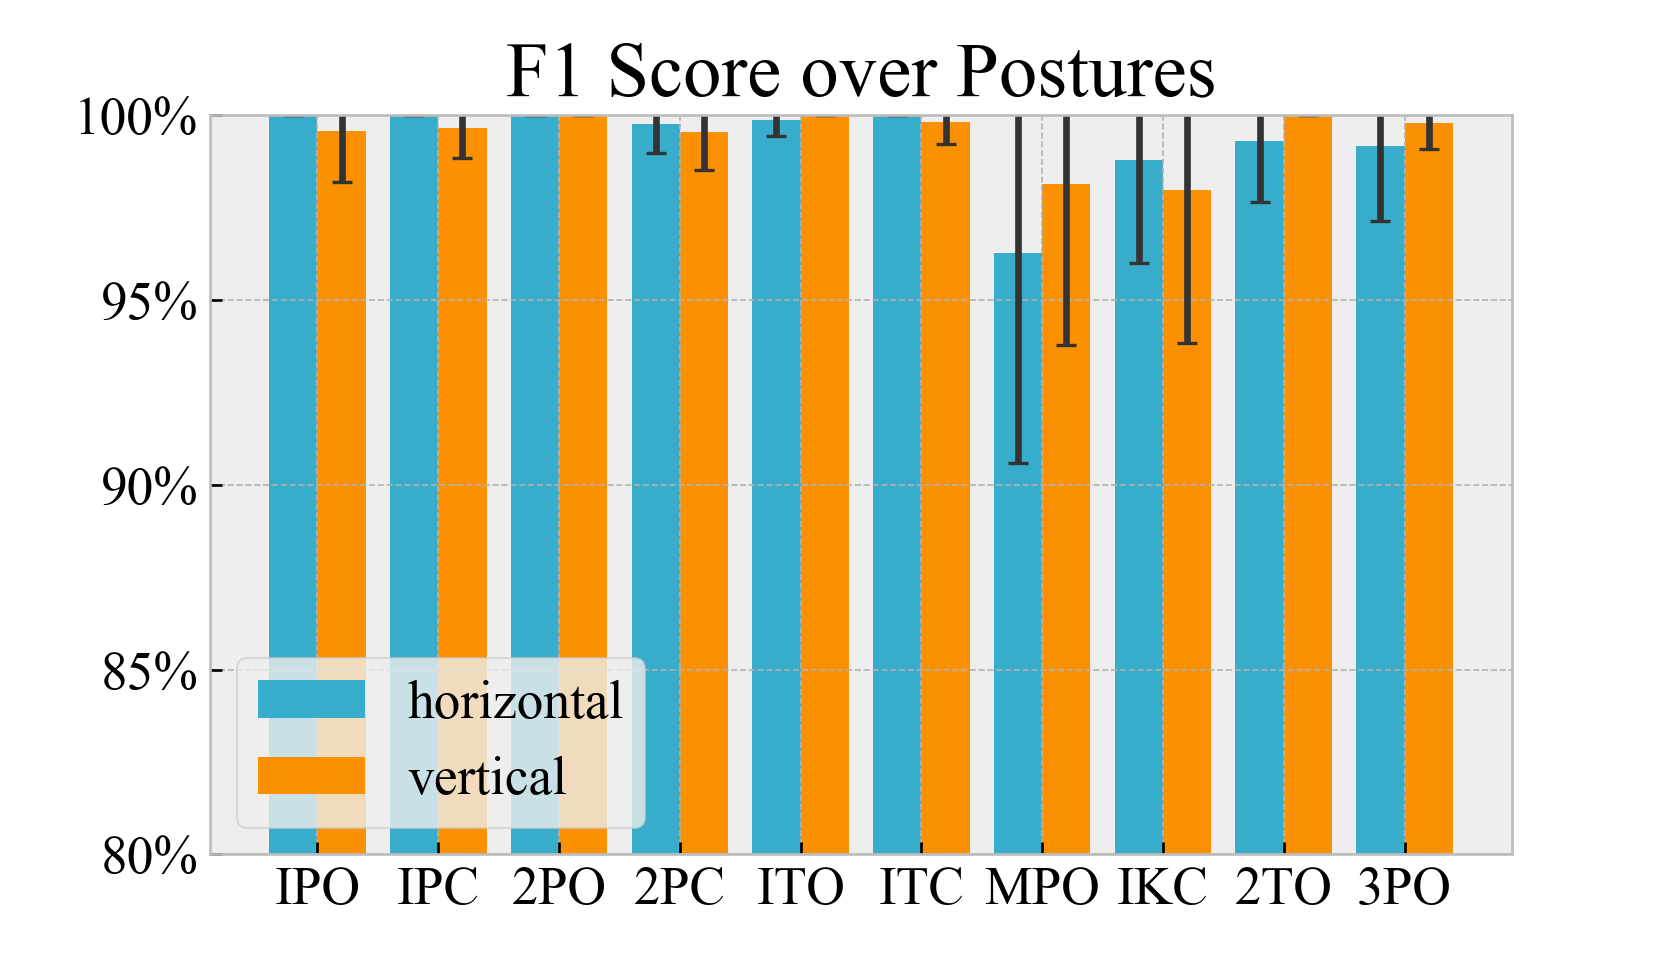
\includegraphics[width=0.8\linewidth]{acc_over_postures.png}
	\caption*{图中展示了触摸检测分类器对十种常用触摸姿态的触摸事件检测准确率,其中误差线表示标准差。}
	\caption{分类器对各触摸姿态的检测准确率}
	\label{fig:acc_over_postures}
\end{figure}

图\ref{fig:acc_over_postures}展示了不同触摸姿态下触摸检测的准确率(F1综合评价指标)。当被试执行敲击姿态MPO(中指指腹点击)和IKC(食指第二关节叩击)时,准确率超过95\%,其它触摸姿态的触摸事件检测准确率均接近100\%。这一结果说明,佩戴在食指上的惯性传感指环在感知食指触摸产生的震动时十分灵敏,而在感知其它手指触摸产生的震动时灵敏度有所下降,但其准确率仍然是可以接受的。

实验者设计了两种基线技术(baseline)用于与本小节所介绍的触摸检测技术做对比,这两种技术分别是基于震动和阈值的方法,和基于视觉的方法:(1)实验者仿照先前工作\cite{lam2002mids, oh2017anywheretouch}实现基于震动和阈值的触摸检测技术,并通过对本章所用数据集进行模拟实验来找到技术中所涉及参数的最优阈值;(2)实验者仿照先前工作\cite{newcombe2011kinectfusion, wilson2010combining, xiao2016direct, xiao2018mrtouch}实现了基于视觉方法的触摸检测技术,当摄像头检测到手指指尖与交互表面的距离下降到10毫米以下时,即汇报触摸事件。图\ref{fig:acc_vs_baseline}现实了本小节所介绍方法与两种基线技术之间的对比,方差分析表面本方法显著提高了触摸检测的精准率($F_{1,11}=10.4,p<.001$)和召回率($F_{1,11}=59.8,p<.0001$, $F_{1,11}=124.7,p<.0001$)。

\begin{figure}
	\centering
	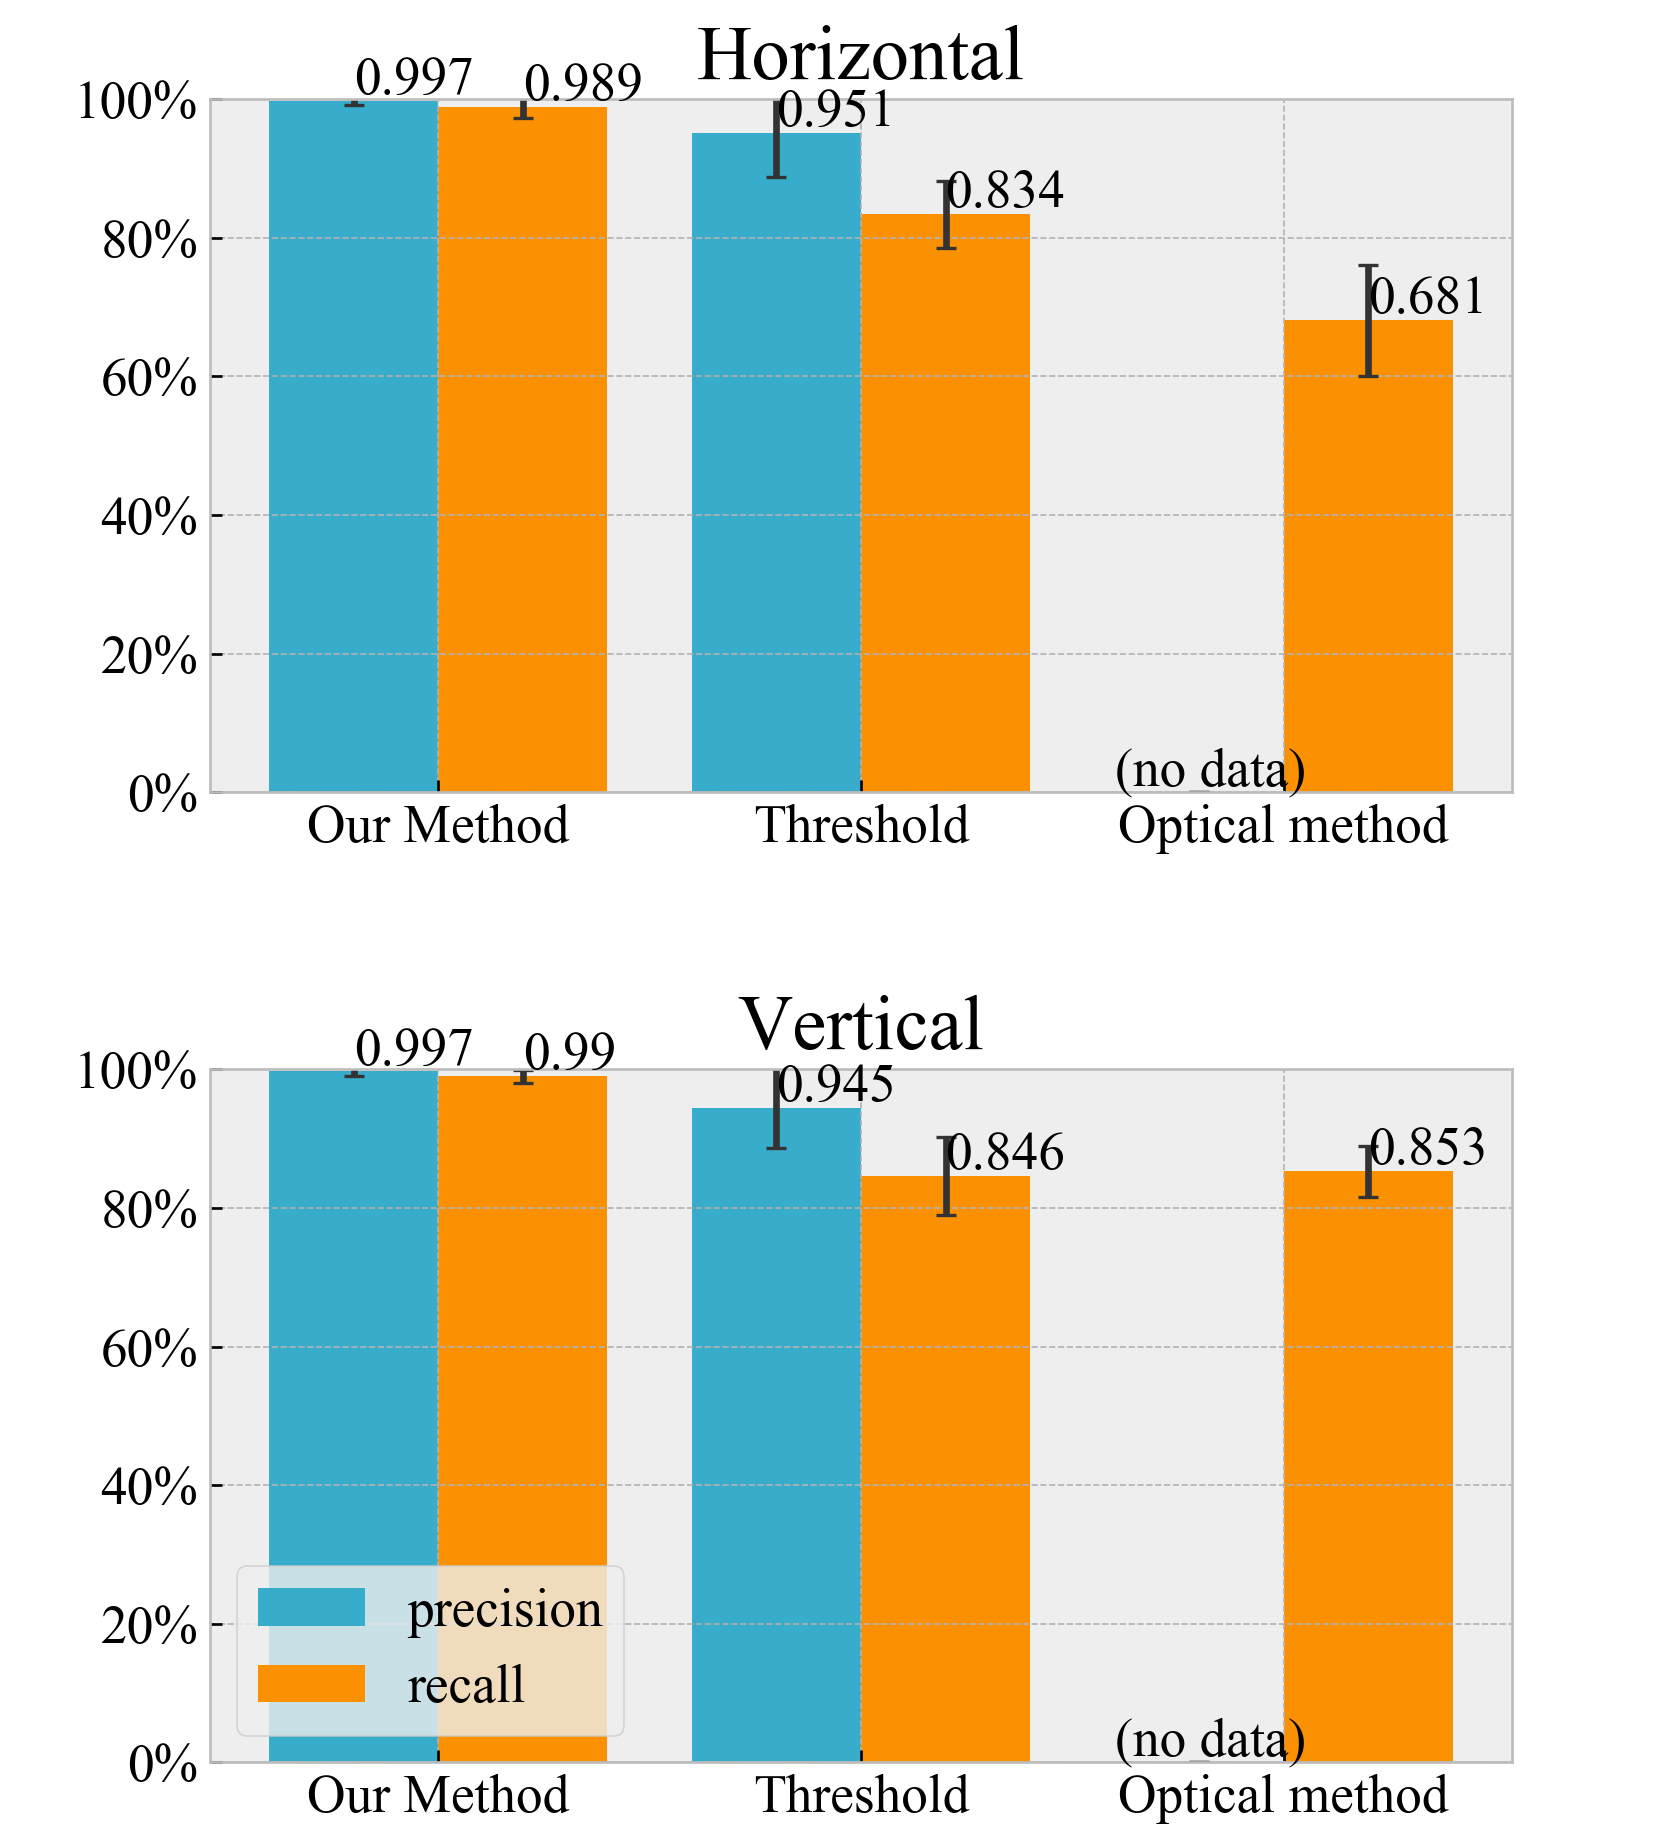
\includegraphics[width=0.8\linewidth]{acc_vs_baseline.png}
	\caption*{图中展示了本触摸检测技术在平均精准率和召回率上的对比,其中,误差线表示标准误差。实验中没有负样本可用于评测视觉方法的精准率。}
	\caption{本触摸检测技术与baseline的对比}
	\label{fig:acc_vs_baseline}
\end{figure}

\subsubsection{触摸检测算法流程}

触摸检测分类器只能就一段惯性传感信号,判断当前是否发生了触摸事件,然而,该分类器还不足以实时感知触摸,这是因为:(1)若时刻通过分类器判断触摸事件,分类器将在手指触摸交互表面后重复报告多次触摸事件;(2)虽然分类器的预测准确率高达99.3\%,但是传感器的运行频率为200赫兹,即每秒钟会调用200次分类器进行判断,这样一来误触的概率还是很大的。为了解决上述问题,实验者设计了一种基于触摸检测分类器的触摸检测算法:

\begin{itemize}
\item 如果在过去的十帧(50毫秒)内分类器预测过触摸事件,则算法不会重复报告触摸事件。
\item 只有当分类器连续两帧判定为触摸时,算法才会报告触摸事件。
\end{itemize}

上述算法会让检测延迟多一帧,但是,它能够大大降低误触的概率,并且不会重复报告多次触摸事件。本章将在实验三中通过实际的触摸交互任务评测该触摸检测算法的性能。

本小节介绍了基于支持向量机(SVM)的触摸检测技术,该方法只是简单版本的触摸检测技术,其目的在于探索清楚基于惯性传感指环的触摸交互技术中的诸多位置问题,为基于触摸运动模型的触摸交互技术打下基础。本小节所得出的结论如下所述:首先,先前工作中采用阈值方法判断触摸事件的方式是低效的,惯性传感指环能提供非常多有用的信息,用于支持低延迟的触摸检测技术;其次,将惯性传感指环佩戴在食指或中指的第一指骨上是最佳选择,该指环佩戴位置既符合用户的主观偏好,有能保证最高的触摸检测准确率;第三,触摸导致的震动能在10毫秒内传递到接触交互表面的手指上,能在20毫秒内传递到相邻手指上。其中,接触交互表面的手指的震感强烈,相邻手指第一指骨上的震感也强烈,但是相邻手指第三指骨处的震动已经不足以支撑高准确率的触摸检测了。上述结论为下一节内容,基于触摸运动模型的低延迟触摸检测技术奠定基础。

\section{基于触摸运动模型的触摸检测技术}

\subsection{基于触摸运动模型的触摸检测技术}\label{section:model_TappingRing}

基于触摸运动模型的触摸检测技术适用于运动传感信号,包括位移、速度和加速度信号。其中,基于摄像头的视觉方法可传感位移信号,惯性传感器可收集加速度信号。本章所提出的MR头盔加上惯性传感指环的智能设备系统可以获取触摸运动的位移和加速度信号,可用于支持低延迟触摸检测技术。本小节将分三种传感信道的情况讨论触摸运动模型如何指导触摸检测技术,这三种情况分别是:(1)仅有位移传感信号;(2)仅有加速度传感信号;(3)融合位移和加速度信号。

\textbf{(1)若仅有位移传感信号}:在追踪手指的过程中,设当前时刻的时间为$t_{now}$,用$t\in[t_{now}-60,t_{now}-10]$毫秒时间内的位移信号拟合无约束运动方程$x(\tau)=x_0+(x_1-x_0)(6\tau^5-15\tau^4+10\tau^3)$,使用信赖阈方法\cite{conn2000trust}进行拟合,若拟合成功,则说明此时手指正处于无约束运动过程中,需要观察手指是否停止运动,以判断手指是否接触到了交互表面。若当前位移测量值$x_m(\tau_{now})$与运动方程的预测值$x(\tau_{now})$相差超过传感信号的三倍标准误差时,可判定触摸事件发生:

\begin{equation}
	\lvert x_m(\tau_{now})-x(\tau_{now})\rvert>3\sigma_x
	\label{equ:touch_condition_x}
\end{equation}

若在成功拟合无约束运动方程后,始终不发上述公式所述情况,说明人的手指做出了空中点击的动作,而非真正的触摸点击。实验表明,触摸瞬间手指速度的经典值为$0.15m/s$,若位移传感信号的标准误差为0.5毫米,则根据上述公式,触摸事件的检测延迟为10毫秒左右。

\textbf{(2)若仅有加速度传感信号}:在记录手指加速度的过程中,设当前时刻的时间为$t_{now}$,用$t\in[t_{now}-60,t_{now}-10]$毫秒时间内的加速度信号拟合无约束运动的加速度方程$a(\tau)=(x_1-x_0)(120\tau^3-180\tau^2+60\tau)$,使用SLSQP算法进行拟合,若拟合成功,则说明此时手指正处于无约束运动过程中,需要观察手指运动是否达到一个很大的加速度,以判断手指是否接触到了交互表面。若当前加速度测量值$a_m(\tau_{now})$与运动方程的预测值$a(\tau_{now})$相差超过传感信号的三倍标准误差时,可判定触摸事件发生:

\begin{equation}
	\lvert a_m(\tau_{now})-a(\tau_{now})\rvert>3\sigma_a
	\label{equ:touch_condition_a}
\end{equation}

由于触摸运动的位移方程在触摸瞬间$t=t_c$不可导,公式揭示此时的加速度无限大。但实际上,手指不是理想的刚体,所以加速度不可能是无限大,而仅仅是相当大。若惯性传感器紧贴在食指的第一关节骨上,它的加速度会在碰撞发生后的10毫秒内达峰值,触摸事件的检测延迟应为10毫秒左右。

\textbf{(3)融合位移和加速度传感信号}:

若同时有位移信号和加速度信号,可以融合两种信号,在保持准确率不变的情况下降低触摸事件检测的延迟。在当前时刻$t_{now}$,位移信号服从正态分布$N(x(\tau_{now}),\sigma_x)$,设位移信号的概率密度函数为$f_x(x_m(\tau_{now}))$:

\begin{equation}
	f_x(x_m(\tau_{now}))=\frac{1}{\sqrt{2\pi}\sigma_x}exp\left(-\frac{(x_m(\tau_{now})-x(\tau_{now}))^2}{2\sigma_x}\right)
\end{equation}

同理,设加速度信号误差的概率密度函数为$f_a(a_m(\tau_{now}))$,则公式\ref{equ:touch_condition_x}、公式\ref{equ:touch_condition_a}分别对应:

\begin{equation}
	\int_{\lvert x_m(\tau_{now})-x(\tau_{now})\rvert<3\sigma_x}f_x(x_m(\tau_{now}))>99.7\%
\end{equation}

\begin{equation}
	\int_{\lvert a_m(\tau_{now})-a(\tau_{now})\rvert<3\sigma_x}f_a(a_m(\tau_{now}))>99.7\%
\end{equation}

由于卡尔曼滤波已经有效利用位移信号和加速度信号的互信息,降低了两者的标准误差,此时可认为位移的误差与加速度的误差相互独立,因此下述公式成立时可判定触摸事件发生:

\begin{equation}
	\int_{\frac{\lvert x_m(\tau_{now})-x(\tau_{now})\rvert^2}{(3\sigma_x)^2}+\frac{\lvert a_m(\tau_{now})-a(\tau_{now})\rvert^2}{(3\sigma_a)^2}<1}f_x(x_m(\tau_{now}))f_a(a_m(\tau_{now}))>99.7\%
\end{equation}

简化以上公式得到,当下述公式成立时可判定触摸事件发生:

\begin{equation}
	\frac{\lvert x_m(\tau_{now})-x(\tau_{now})\rvert^2}{(3\sigma_x)^2}+
	\frac{\lvert a_m(\tau_{now})-a(\tau_{now})\rvert^2}{(3\sigma_a)^2}>1
\label{equ:x_a_judgement}
\end{equation}

以上就是触摸运动模型对触摸检测技术的计算理论指导,根据上述数学推导,接下来将介绍触摸检测的算法流程:

\begin{enumerate}
\item 通过摄像头和视觉的方法实时采集用户手指的位移信号,通过佩戴在手指上的惯性传感指环采集手指的加速度信号,每一时刻都截取从当前时刻往前推100毫秒内的信号数据,作后续处理。
\item 根据Madgwick算法\cite{madgwick2010efficient}计算指环加速度信号在重力方向上的投影,然后根据第二章所介绍的触摸运动模型的计算方法,拟合当前的无约束运动方程,若拟合成功,则说明此时手指正处于无约束运动过程中,跳至下一步骤。
\item 开始检测手指的位移和加速度信号是否满足公式\ref{equ:x_a_judgement},若满足,则判定触摸事件已发生,若在无约束运动方程拟合成功后20毫秒内,公式\ref{equ:x_a_judgement}未得到满足,则回到上一步骤
\end{enumerate}

以上就是基于触摸运动模型的触摸检测算法,接下来一节将通过真实的触摸交互任务评测本技术,同时对比本小节中提到的一系列初探的或先前工作的触摸检测技术。

\subsection{实验三:评测本节触摸检测技术}

本实验通过实际的触摸交互应用程序评测本章所提出的触摸检测技术,实验共对比了三种不同的触摸检测技术,分别是:(1)基线(baseline)技术,先前工作中基于视觉的触摸检测技术\cite{xiao2018mrtouch};(2)本章第3.7节中介绍的,基于机器学习的触摸检测技术;(3)本章第3.8节中介绍的,基于触摸运动模型的低延迟触摸检测技术。为了让上述技术在尽可能苛刻的条件下接受评测,实验者选取了一款名为“别碰白键”的游戏作为实验的交互任务,该游戏要求玩家进行尽可能快速的连续触摸点击。

\subsubsection{实验设计和过程}

实验者从校园中招募了12名被试,其中3名为女性,被试的年龄从20岁到28岁不等,平均年龄为23.2岁。这一批被试未参与之前的任何一个用户实验。实验共分为两大部分,被试分别在水平的桌面和垂直的墙面上进行游戏。每一部分的实验又包含三段实验,每段实验采用不同的触摸检测技术。采取组内实验设计,即每一名被试都要使用不同的触摸检测技术进行实验,为了避免学习效应,实验者采用拉丁方来平衡不同触摸检测技术的实验顺序。

实验中,被试像实验二那样佩戴惯性传感指环,同时,在头上佩戴手型追踪摄像头LeapMotion,实验设置图同实验二的\ref{fig:tapping_ring_config}。被试将指环佩戴在食指第一关节上,通过最常用的触摸姿态,即食指指腹点击进行触摸交互。如图\ref{fig:tapping_ring_app}所示,本实验在一个显示器上展示了“别碰白键”这款游戏,同时也在游戏中渲染了被试的虚拟手,显控比为1:1。“别碰白键”这款游戏的目标是尽可能快速地通过触摸来点击从屏幕顶部出现的黑色按键,同时避开白色按键。每点中一个黑色按键,新一行的按键就会从屏幕的顶部弹出;如果被试不慎点中了白色按键,屏幕就会闪烁一秒以报告错误。游戏中,被试需要点击100个黑色按键来结束游戏,游戏的目标是尽快点击完这100个黑色按键。

\begin{figure}
	\centering
	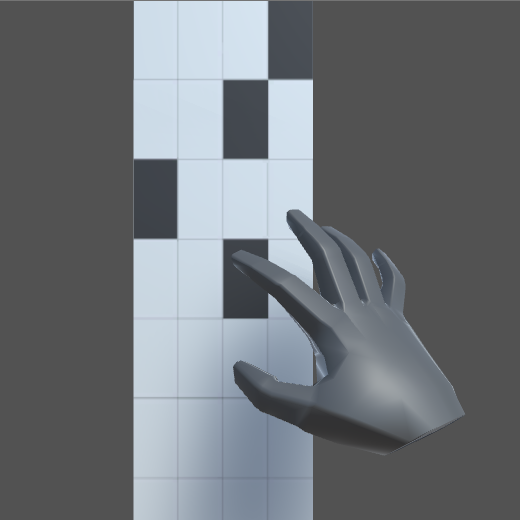
\includegraphics[width=0.6\linewidth]{tapping_ring_app.png}
	\caption*{图中所示为本实验的交互任务:别碰白键,这是一款要求用户以尽可能快的速度进行连续触摸的游戏,能够有效测试触摸检测技术的性能。}
	\caption{实验任务图示}
	\label{fig:tapping_ring_app}
\end{figure}

本实验的总时长为20分钟,我们通过触摸检测的准确率、延迟,和用户完成任务的时间来评价三种不同触摸测试技术的性能。

\subsubsection{实验结果}

\begin{table}[!htbp]
	\centering
	\begin{tabular}{l|lll}
		\toprule
		& 基于视觉方法\cite{xiao2018mrtouch}  & 基于机器学习 & 基于触摸运动模型 \\
		\midrule
		精准率 & 85.42\%(10.42\%) & 98.62\%(2.50\%) & 99.32(0.74\%) \\
		召回率 & 84.08\%(9.24\%) & 98.61\%(1.33\%)  & 99.17(0.88\%) \\
		任务完成时间(秒) & 44.30(19.19) & 35.74(13.69) & 36.21(14.82) \\
		检测延迟(毫秒) & 5.48(15.07) & 9.11(3.41) & 9.02(3.16) \\
		\bottomrule
	\end{tabular}
	\caption{表格对比了不同触摸检测技术的性能,括号中的数值为标准差。}
	\label{tab:tapping_ring_study3}
\end{table}

%请注意,表中的延迟是所评测技术的延迟和低延迟触摸板测量值(本实验的真值)之间的差距。因此实际延迟还可能多0到5毫秒,来至低延迟触摸板的延迟。

表\ref{tab:tapping_ring_study3}展示了实验的评测结果。在检测准确率(F1综合评价指标)方面,方差分析表明,无论是基于触摸运动模型的触摸检测技术($F_{1,11}=87.9,p<.001$),还是基于机器学习的方法($F_{1,11}=53.6,p<.001$),都显著优于先前工作中基于视觉的方法。通过分析视觉方法中的错误案例能发现,本实验的交互任务要求被试连续快速触摸,基于视觉的方法不能很好的处理这种情况,例如,基于视觉的方法认为手指离开交互表面超过15毫米才算一次触摸动作完成,但在连续快速触摸任务中,连续两次触摸之间被试的手指可能从未离开交互表面超过15毫米,这影响了第二次触摸事件的检测。而在本章所提出的两种触摸检测技术的比较中,基于触摸运动模型的触摸检测技术的准确率超过99\%,显著高于基于机器学习方法的准确率($F_{1,11}=5.6,p<.05$)。数据分析发现,这一差异主要来源于对较轻的触摸的检测,基于触摸运动模型的触摸检测技术检测更准确,这可能是因为基于模型的方法更好地利用了触摸之前手指向下运动的信息。

在被试完成实验任务的时间方面,方差分析表明,基于触摸运动模型的触摸检测技术($F_{1,11}=7.9,p<.05$)和基于机器学习的方法($F_{1,11}=8.3,p<.05$),都显著优于先前工作中基于视觉的方法。这是因为在视觉方法中,过高的检测错误率让被试经常需要纠正错误,延误了完成任务的时间。而在本章所提出的两种触摸检测技术的比较中,被试完成任务的时间没有显著性差异。

在检测延迟这方面,基于机器学习或触摸运动模型的触摸检测技术的延迟都稳定在10毫秒以内。而基于视觉的方法的检测延迟则非常不稳定,从表格中可以看到,视觉方法的检测延迟平均值为5.48毫秒,但是其标准差却高达15.07毫秒。有的时候视觉方法甚至会提前汇报触摸事件,导致负延迟的情况,这是因为视觉方法规定,当手指与交互表面下降到10毫米阈值以下时,即报告触摸事件。采访被试发现,没有被试能在基于机器学习或触摸运动模型的触摸检测技术下察觉到延迟的存在,但在基于视觉方法的技术中,则能明显感受到延迟忽快忽慢。

综合上述实验结果,基于触摸运动模型的触摸检测技术具有很高的检测准确率,显著高于先前工作,也显著高于基于简单机器学习的方法。而在检测延迟这方面,基于触摸运动模型的触摸检测技术也显著优于先前工作。这说明,基于惯性传感指环的触摸检测技术很具有实用前景,值得更多的关注。

\section{本章小结}

任意无源表面上的触摸交互很可能是未来的一种主要人机交互方式,头戴式混合现实系统可以在普通物体表面上叠加交互界面,使得这些物体表面上的触摸交互成为可能。先前工作已经提出利用MR头盔的前置摄像头跟踪手型\cite{xiao2018mrtouch},但是相关工作在判断手指是否接触到交互表面上时遇到了困难。本章内容是第一份专注于优化惯性传感指环触摸检测技术的研究。评测结果表明,基于触摸运动模型的指环触摸检测技术可以在10毫秒以内的低延迟下检测触摸事件,召回率高达99.17\%,误触率仅为0.68\%。低延迟是本触摸交互技术的核心贡献之一,这是因为,人在触摸交互中无法察觉到低于24毫秒的延迟\cite{jota2013fast},而本技术的延迟仅为10毫秒,在响应性上提供了最佳的用户体验。从原理的角度来看,基于触摸运动模型的触摸检测技术性能更优有其底层逻辑:(1)触摸运动模型充分利用了多帧信息,降低单帧信号误差带来的影响;(2)无需直接观测触摸点,有效回避视觉遮挡问题\cite{xiao2018mrtouch}。
